The name flow following comes from the monograph \cite{ElmSilWat14}.\td{\textbf{fix}: the notation of the matrix entries in this subsection needs to be adapted to fit the rest of the chapter.}

It is well known that the performance of the GMRES method \cite{Gre97} when
applied to problems treated in this thesis is governed by a period of slow initial convergence
followed by a rapid decrease of the relative residual norms \cite{LieStr03-2}.
Numerical experiments show that the use of ``flow-following" preconditioners
\cite{ElmSilWat14} eliminates the stagnation phase leading to fast convergence
in only a few steps (see Figure \ref{fig:back:1DConvergence}). These preconditioners
originate from multi-step stationary iterative methods, where each intermediate
step corresponds to a renumbering of the unknowns which tries to follow the
flow, i.e. tries to go in the direction of the dominating convection, in
different parts of the domain.

The traditional analyses of stationary iterative methods (e.g., Jacobi,
Gauss-Seidel, SOR) based on the spectral radius of the system matrix $\A$ do not
provide insight into renumbering issues \cite{Eie93}; even though the
spectral radius is the same for different orderings of the unknowns and it is
independent of the signs of the convection terms, the method presents different
convergence behaviors for different orderings:
%(see Figure \ref{fig:1D:GSres}[right]).
\begin{figure}[h!]
\centering
%\vspace*{-2em}
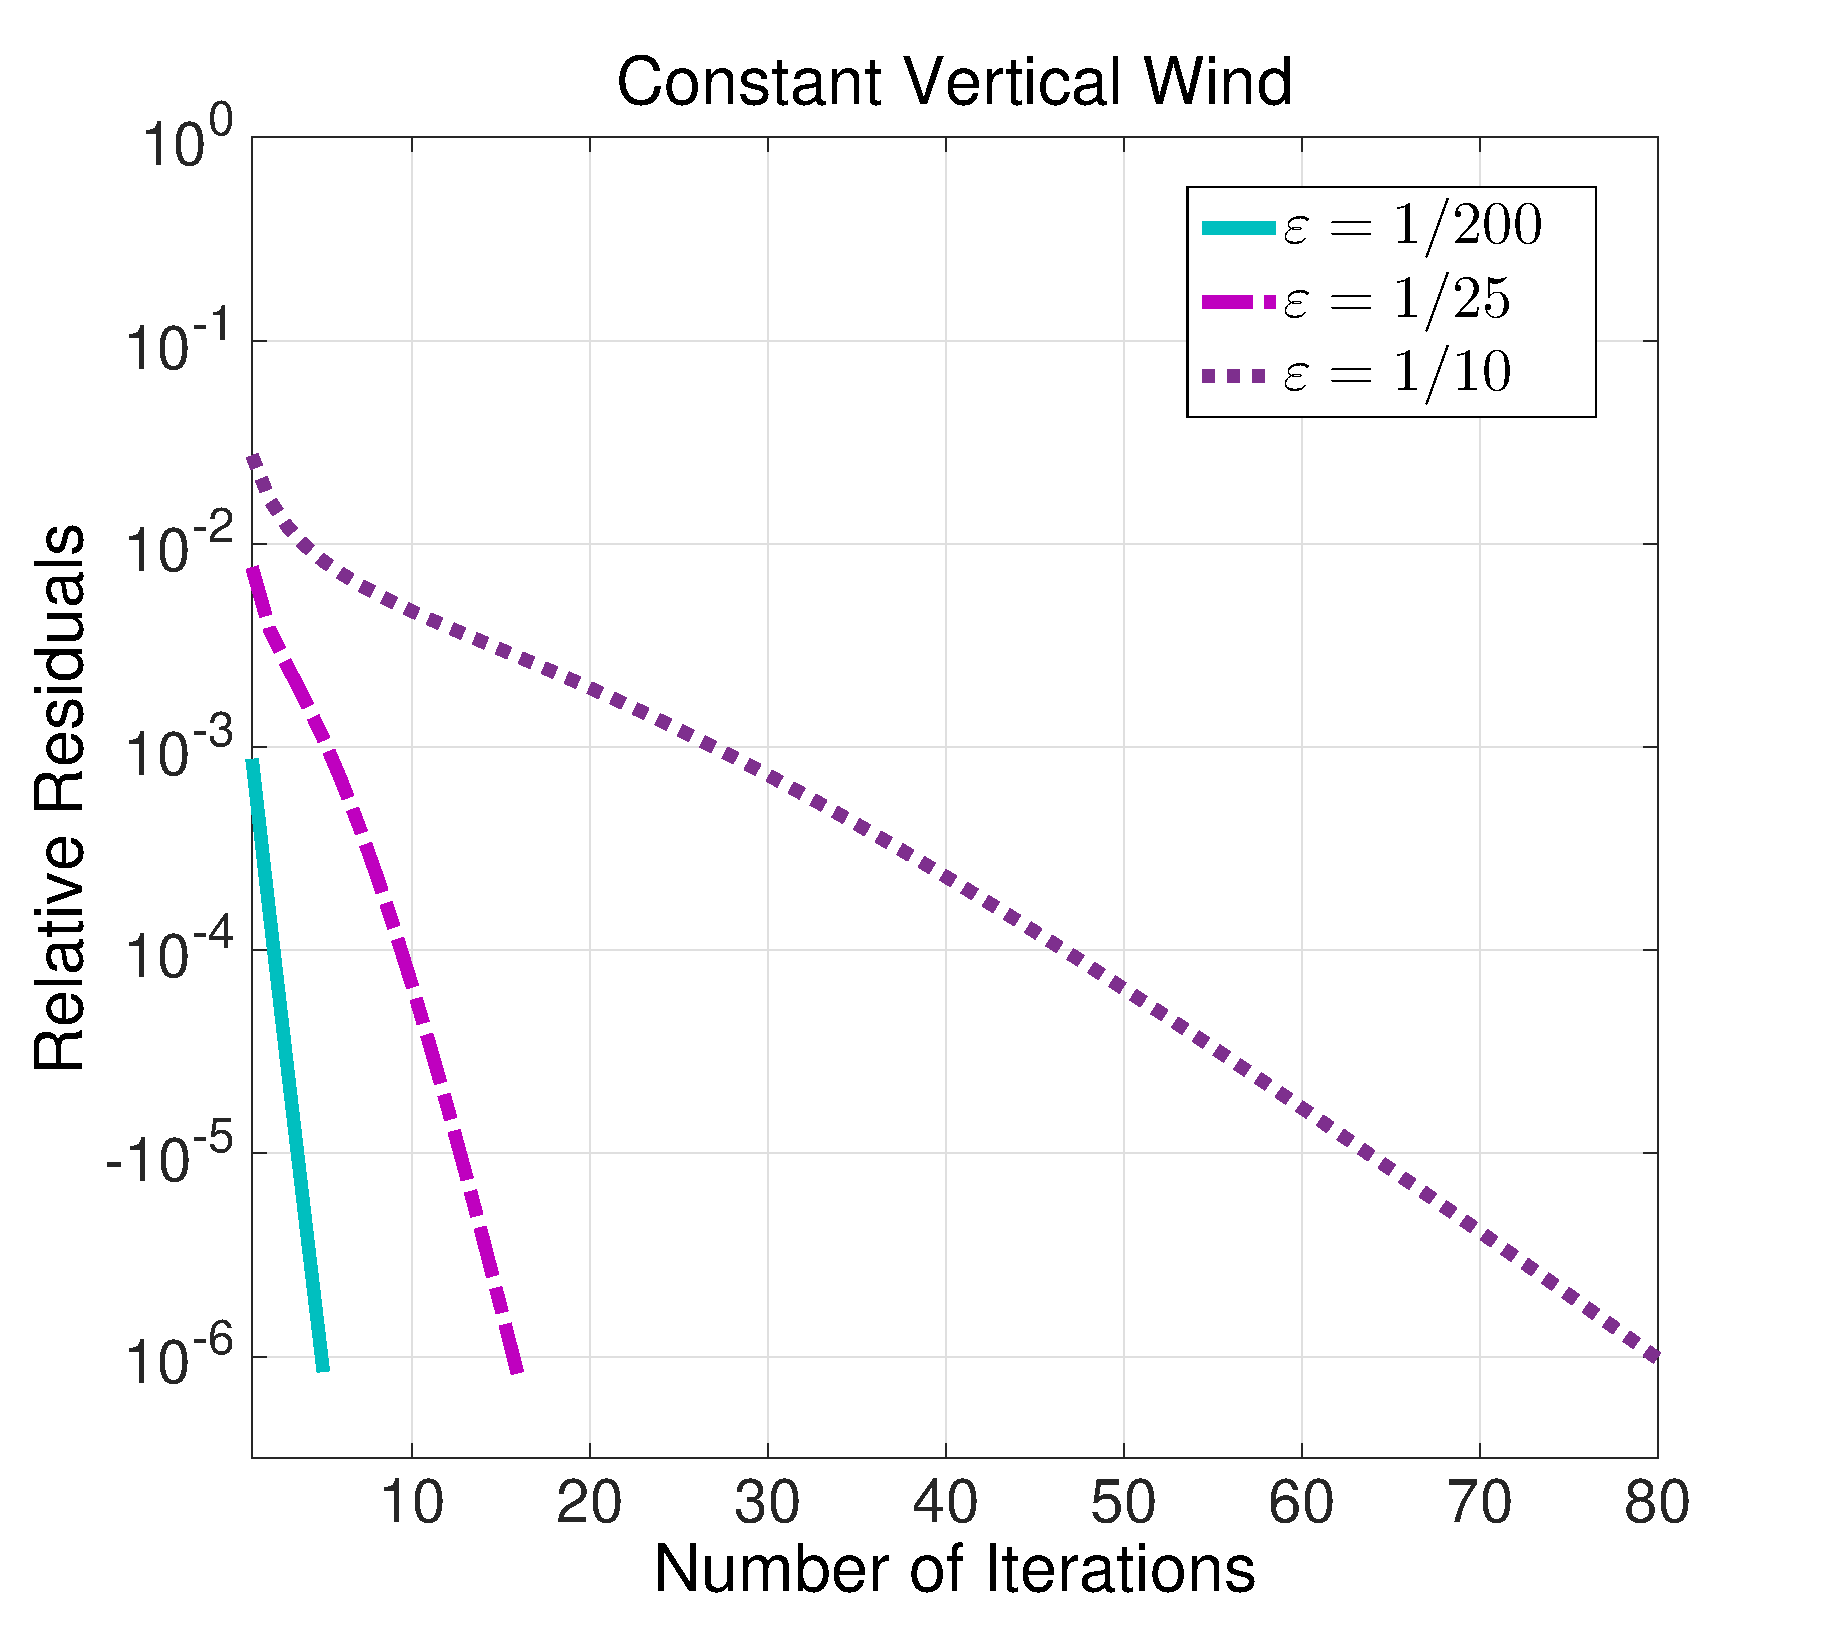
\includegraphics[scale=0.21]{figures/bottom-to-top-GS-vertical-wind}
%\hspace*{-2em}
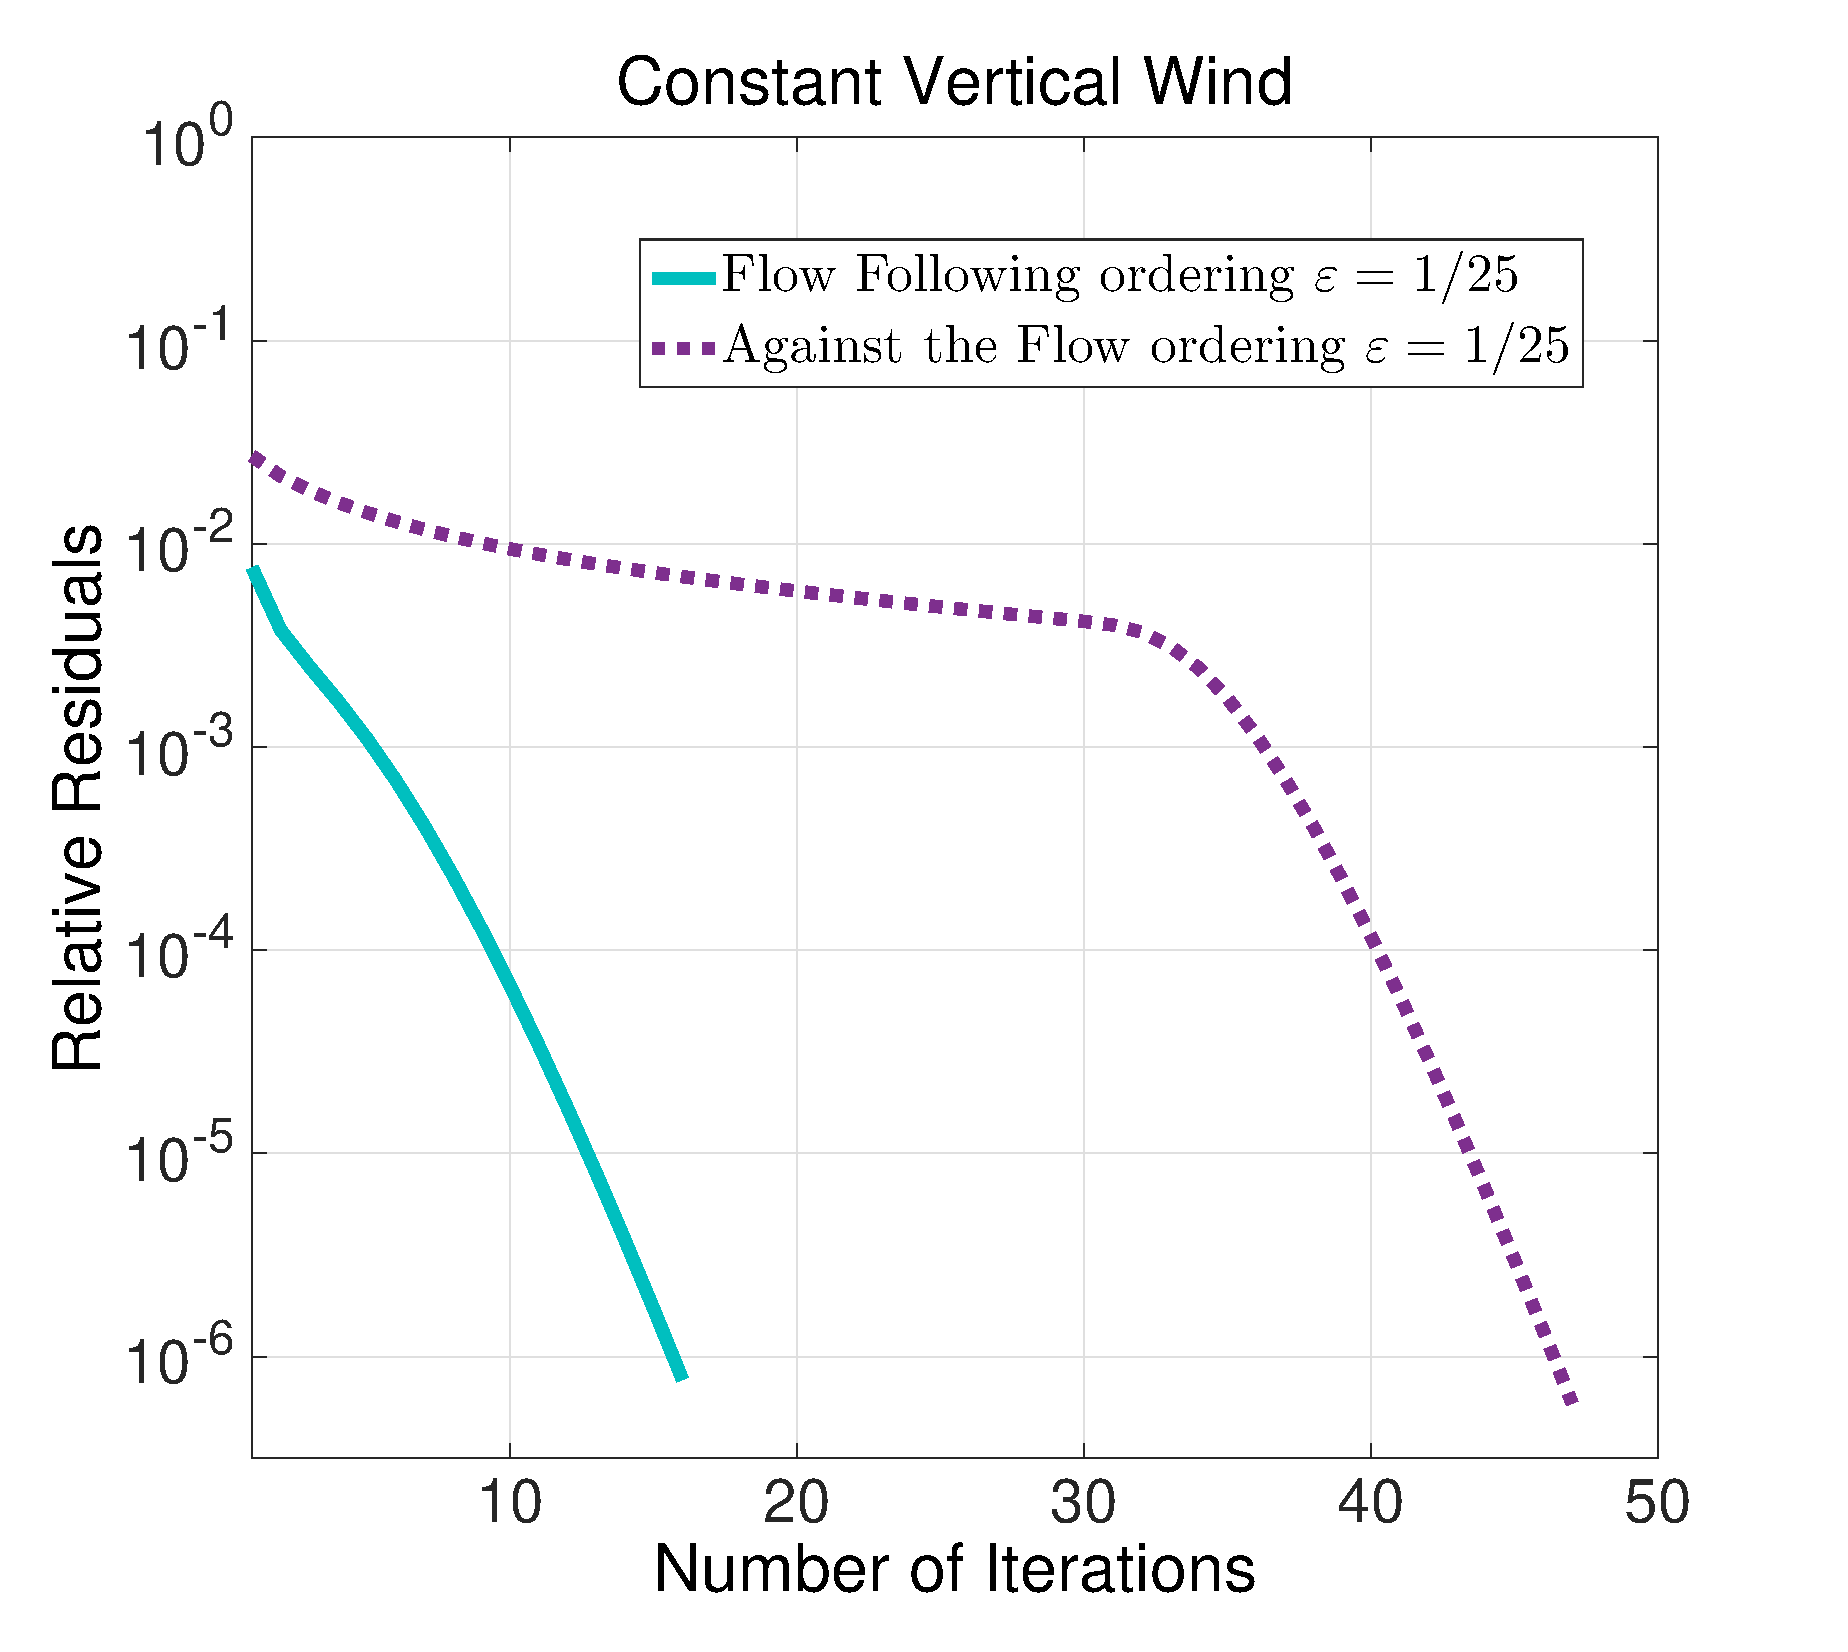
\includegraphics[scale=0.21]{figures/ordering-GS-vertical-wind_eps_25}
%\includegraphics[scale=0.29]{figures/bottom-to-top-GS-30-degree-wind}
%\vspace*{-1em}
\caption{Relative residuals $\|\mathbf{r}^{(k)}\|/\|\mathbf{f}\|$ vs iteration
numbers for stationary Gauss-Seidel solution of discrete systems of constant
vertical wind. Dependence on perturbation parameter [left]. Dependence on
numbering of the unknowns [right].[Reproduced from experiments in
\cite{ElmSilWat14}]}
%\caption{Relative residuals $\|\mathbf{r}^{(k)}\|/\|\mathbf{f}\|$ vs
%Iteration
%numbers for stationary Gauss-Seidel solution of discrete systems of constant
%vertical wind [Left] and constant wind @ 30 degree angle [Right], for
%$\mathbf{Q}_1$ approximation, $32\times32$ square grids and streamline
%diffusion discretization. [Reproduced from experiments in \cite{Elman2006}]}
\label{fig:1D:GSres}
\end{figure}
%
In other words, the spectral radius is a measure of the asymptotic
speed of convergence of such methods but provides no information about the
transient behavior. A different, more descriptive, approach is proposed in
\cite{ElmChe93}, where bounds for the $\infty$-norm, $1$-norm, and $2$-norm
of the iteration matrices of the stationary scheme are derived and used to
bound the convergence history of the Gauss-Seidel method from early stages of
the solution process.

In this paper we use the splitting operator $(\M_S)$ corresponding to a
multi-step stationary iterative method (relaxation scheme), as a preconditioner
for the discrete operator $\A$ and apply the GMRES method to the preconditioned
system
\begin{equation}\label{eq:1D:precls}
\M_S^{-1}\A \u_h = \M_S^{-1}\f_h.
\end{equation}
%or in right-preconditioning form
%\[
%	A M^{-1} g_h= f_h,\quad g_h=Mu_h.
%\]
Based on the convergence analysis found in \cite{ElmChe93}, we present
bounds on the norm of the multi-step iteration matrix $(\S)$ which, in turn, are
used to bound the residual minimization history of the GMRES method using the
equivalence:
\[\S=\I-\M_S^{-1}\A.\]

\subsubsection{Bounding the norm of the iteration matrix}
Recall that at step $k$ the GMRES method applied to \eqref{eq:1D:precls} solves
the residual minimization problem
\begin{equation}\label{eq:1D:gmres}
\|\r_k\|_2 = \min_{p \in \Pi_{k} }\|p_k(\M_S^{-1}\A)\r_0\|_2
\end{equation}
where $\Pi_{k}$ denotes the set of  polynomials of degree less than $k$ such
that $p(0)=1$. Thus, fast convergence of GMRES is expected if
$\|\I-\M_S^{-1}\A\|$
is small, see \cite[p. 56]{Gre97}.
From the expression \eqref{eq:1D:gmres} one derives the relative residual bound
\begin{equation}\label{eq:1D:resboundmeth3}
\frac{\|\r_k\|}{\|\r_0\|} \leq \min_{p \in \Pi_k} \|p_k(\M_S^{-1}\A)\|_2 \leq
\|(\I-\M_S^{-1}\A)^k\|_2
\end{equation}
by choosing $p(x) = (1-x)^{k} \in \Pi_{k}$ and noting that it is an admissible
GMRES polynomial.

Since for the FGS method $(\I~-~\M_F^{-1}\A)^k~=~\F^k$, the right term can be
bounded using the bounds derived in \cite[Section 5]{ElmChe93}. We will
first compute the bounds for the $\|\cdot\|_\infty$ and $\|\cdot\|_1$ norms and
show that they also hold for $\|\cdot\|_2$ (this is explained at the end of
that paper). In the following, we derive expressions for the entries of the
matrices $(\I~-~\M_S^{-1}\A)^k$, i.e., when the SGS preconditioner is used instead
of the FGS preconditioner. By introducing the notation $\llbracket \cdot
\rrbracket$, where  $\llbracket \cdot \rrbracket=1$ if the expression $\cdot$
is true, and $0$ otherwise, the following theorem, provides an analytic
expression for the elements of the matrix $\S$ in terms of the entries of the
unpreconditioned matrix. Further on,  this expression will be used to bound the
norm of the GMRES residuals.

\begin{thm}\label{thm:1D:matSentries}
The entries of the SGS iteration matrix, $\S$, are given by
\begin{equation}\label{eq:1D:Smatentries}
[\S]_{ij}=%e_i^TSe_j=
\llbracket j>1\rrbracket \cdot
\left(\frac{d}{d-1}\right)c^{-i}b^{-j}\left[d^{n+1}-d^{\max(i,j)} \right],
\end{equation}
where $d=bc$.
\end{thm}
\begin{proof}
We derive expressions for the elements of the SGS method's iteration matrix (as
well as expressions for intermediate relevant quantities) by expressing the
matrices $\M_F$, $\M_B$, $\N_F$, etc. in terms of the nilpotent shift matrix
 of order $n$
 \begin{equation*}
\Z=[\e_2,\ldots,\e_N,0]  =
\left[
\begin{array}{cccc}
0 & & &\\
1 & 0  & & \\
 & \ddots & \ddots & \\
& & 1 & 0
\end{array}
\right].
\end{equation*}

The shifting property of the matrix $\Z$ and its transpose can be seen by its
action on the canonical basis vectors, we have
%
\begin{equation}\label{eq:1D:shift}
\Z\e_j=\begin{cases}
0 &\mbox{if } j=n, \\
\e_{j+1}& \mbox{if } 1 \leq j < n,
\end{cases}
\quad\text{ and }\quad
\Z^T\e_j=\begin{cases}
0 &\mbox{if } j=1, \\
\e_{j-1}& \mbox{if } 1 < j \leq n,
\end{cases}
\end{equation}
%
and for all its powers $t>1$,
%
\begin{equation}\label{eq:1D:shiftk}
\Z^t\e_j=\begin{cases}
\e_{j+t} &\mbox{if } 1 \leq j \leq n-t, \\
0 & \mbox{otherwise},
\end{cases}
\quad\text{ and }\quad
(\Z^T)^t\e_j=\begin{cases}
\e_{j-t} &\mbox{if } t < j \leq n, \\
0 & \mbox{otherwise}.
\end{cases}
\end{equation}
%
Using equation \eqref{eq:1D:shift}, the action of the matrices $\L$ and $\U$
becomes evident,
\begin{equation*}
\L\e_j=b\Z\e_j=b\e_{j+1}\cdot\llbracket j<n \rrbracket,
\quad\text{ and }\quad
\U\e_j=c\Z^T\e_j=c\e_{j-1}\cdot\llbracket j>1 \rrbracket.
%Le_j=bSe_j=
%\begin{cases}
%0 &\mbox{if } j=n \\
%be_{j+1}& \mbox{if } 1 \leq j < n,
%\end{cases}
%\quad\text{ and }\quad
%Ue_j=cS^Te_j=\begin{cases}
%0 &\mbox{if } j=1 \\
%ce_{j-1}& \mbox{if } 1 < j \leq n,
%\end{cases}
\end{equation*}
%
Since the matrices $\Z$ and $\Z^T$ are nilpotent of order $n$, we can express
the inverse of the matrices $\M_F$ and $\M_B$ as truncated Neumann series
expansions. For the matrix $\M_F$, we have
\begin{equation*}
\M_{F}^{-1} = (\D-\L)^{-1} = (\I-b\Z)^{-1} = \sum_{t=0}^{\infty}(b\Z)^{t} =
\sum_{t=0}^{n-1} b^t(\Z)^{t},
\end{equation*}
and its action on the canonical vectors is then
\begin{equation*}
\M_{F}^{-1}\e_j = \sum_{t=0}^{n-1} b^t(\Z)^{t}\e_j =
\begin{cases}
\e_{n} &\mbox{ for } j=n, \\
\sum_{t=0}^{n-j} b^t\e_{j+t}=\sum_{k=j}^{n}
b^{k-j}\e_{k}=b^{-j}\sum_{k=j}^{n}b^{k}\e_{k}, & 1\leq j<n,
\end{cases}
\end{equation*}
%
where we have used the change of variable $k=j+t$. Its entries are thus given
by
\begin{equation*}
\e_i^T\M_{F}^{-1}\e_j =
\begin{cases}
1\cdot\llbracket i=n \rrbracket &\mbox{ for } j=n, \\
b^{-j}\sum_{k=j}^{n}b^{k}\e_i^T\e_{k}= b^{-j}b^{i}\cdot\llbracket i\geq
j\rrbracket=b^{i-j}\cdot\llbracket i\geq j\rrbracket, &\mbox{ for } 1\leq j<n.
\end{cases}
\end{equation*}
%
Now, the action of the iteration matrix of the FGS method, $\F$, is given by:
\begin{equation*}
\F\e_j=\M_F^{-1}\U\e_j=c\M_F^{-1}\Z^T\e_j=c\M_F^{-1}\e_{j-1}\cdot\llbracket
j>1\rrbracket=
cb^{1-j}\sum_{k=j-1}^{n}b^{k}\e_{k}\cdot\llbracket j>1 \rrbracket,
\end{equation*}
%\begin{equation}
%Fe_j=M_F^{-1}Ue_j=cM_F^{-1}S^Te_j=cM_F^{-1}e_{j-1}=
%\begin{cases}
%0 &\mbox{ for } j=1 \\
%cb^{1-j}\sum_{k=j-1}^{n}b^{k}e_{k}, & 2\leq j\leq n,
%\end{cases}
%\end{equation}
%and its entries by
%
\begin{equation*}
\e_i^T\F\e_j=
\begin{cases}
0 &\mbox{ for } j=1, \\
cb^{1-j}\sum_{k=j-1}^{n}b^{k}\e_i^T\e_{k}= cb^{1+i-j}\cdot\llbracket i\geq
j-1\rrbracket, & 1< j\leq n.
\end{cases}
\end{equation*}

We can apply the same reasoning for the matrix $\M_B$ and obtain
%
\begin{equation*}
\M_{B}^{-1} = (\D-\U)^{-1} = (\I-c\Z^T)^{-1} = \sum_{t=0}^{\infty}(c\Z^T)^{t} =
\sum_{t=0}^{n-1}c^t(\Z^T)^{t}.
\end{equation*}
Its action on the canonical vectors is then
%
\begin{equation*}
\M_{B}^{-1}\e_j = \sum_{t=0}^{n-1}c^t(\Z^T)^{t}\e_j =
\begin{cases}
\e_{1} &\mbox{ for } j=1, \\
\sum_{t=0}^{j-1} c^t\e_{j-t} = \sum_{k=1}^{j}
c^{j-k}\e_{k}=c^{j}\sum_{k=1}^{j}c^{-k}\e_{k} & 1< j\leq n,
\end{cases}
\end{equation*}
where we have used the change of variable $k=j-t$, and its entries are given by
%
\begin{equation*}
\e_i^T\M_{B}^{-1}\e_j =
\begin{cases}
1\cdot\llbracket i=1 \rrbracket &\mbox{ for } j=1, \\
c^{j}\sum_{k=1}^{j}c^{-k}\e_i^T\e_{k}=c^jc^{-i}\cdot\llbracket i\leq
j\rrbracket=c^{j-i}\cdot \llbracket i\leq j\rrbracket & 1< j\leq n.
\end{cases}
\end{equation*}
%
The action of the iteration matrix of the BGS method, $\B$, is given by
\begin{equation*}
\B\e_j=\M_B^{-1}\L\e_j=b\M_B^{-1}\Z\e_j=b\M_B^{-1}\e_{j+1}\cdot\llbracket j<n \rrbracket=
bc^{j+1}\sum_{k=1}^{j+1}c^{-k}\e_{k}\cdot\llbracket j< n\rrbracket,
\end{equation*}
%\begin{equation}
%Be_j=M_B^{-1}Le_j=bM_B^{-1}Se_j=bM_B^{-1}e_{j+1}=
%\begin{cases}
%0 &\mbox{ for } j=n \\
%bc^{j+1}\sum_{k=1}^{j+1}c^{-k}e_{k}, & 1\leq j< n,
%\end{cases}
%\end{equation}
and its entries by
%
\begin{equation*}
\e_i^T\B\e_j=
\begin{cases}
0 &\mbox{ for } j=n, \\
bc^{j+1}\sum_{k=1}^{j+1}c^{-k}\e_i^T\e_{k}= bc^{1+j-i}\cdot\llbracket i\leq
j+1\rrbracket, & 1\leq j< n.
\end{cases}
\end{equation*}
%

We can use these expressions to calculate the entries of the iteration matrix
of the SGS method, $\S$, given by:
\begin{eqnarray*}
\S\e_j&=&\M_B^{-1}\L\M_F^{-1}\U\e_j=\M_B^{-1}\L\left(cb^{1-j}\sum_{k=j-1}^{n}b^{k}\e_{k} \cdot \llbracket j>1\rrbracket\right)\\
&=&\llbracket j>1\rrbracket \cdot cb^{1-j}\sum_{k=j-1}^nb^k\M_B^{-1}\L\e_k\\
&=&\llbracket j>1\rrbracket \cdot cb^{1-j}\sum_{k=j-1}^nb^k
\left( bc^{k+1}\sum_{s=1}^{k+1}c^{-s}\e_s\cdot  \llbracket k<n \rrbracket
\right)\\
&=& \llbracket j>1\rrbracket \cdot cb^{1-j}\sum_{k=j-1}^nb^{k+1}c^{k+1}\cdot
\llbracket k<n \rrbracket \sum_{s=1}^{k+1}c^{-s}\e_s\\
&=& \llbracket j>1\rrbracket\cdot db^{-j}\sum_{k=j-1}^nd^{k+1}\cdot\llbracket
k<n \rrbracket \sum_{s=1}^{k+1}c^{-s}\e_s.
\end{eqnarray*}
and its entries by
%
\begin{eqnarray*}
\e_i^T\S\e_j
&=&\llbracket j>1\rrbracket \cdot db^{-j}\sum_{k=j-1}^n \llbracket
k<n\rrbracket \cdot d^{k+1}\sum_{s=1}^{k+1}c^{-s}\e_i^T\e_s\\
&=&\llbracket j>1\rrbracket \cdot db^{-j}\sum_{k=j-1}^n \llbracket
k<n\rrbracket \cdot d^{k+1}c^{-i}\cdot\llbracket i \leq  k+1\rrbracket \\
&=&\llbracket j>1\rrbracket \cdot d^2b^{-j}c^{-i}\sum_{k=j-1}^n d^{k}\cdot
\llbracket i-1 \leq  k < n\rrbracket .
\end{eqnarray*}
%There are now two cases which are of importance, mainly $i\geq j$ and $i<j$.
%\begin{eqnarray}
%e_i^TSe_j=
%\begin{cases}
%[j>1]\cdot d^2b^{-j}c^{-i}\sum_{k=i-1}^{n-1} d^{k} &\mbox{ for } i\geq j, \\
%[j>1]\cdot d^2b^{-j}c^{-i}\sum_{k=j-1}^{n-1} d^{k} &\mbox{ for } i<j.
%\end{cases}
%\end{eqnarray}
After simplifying we obtain
\begin{eqnarray*}
\e_i^T\S\e_j=
\begin{cases}
\llbracket j>1 \rrbracket \cdot d^2b^{-j}c^{-i}\left[ \frac{d^{n}-d^{i-1}}{d-1}
\right] &\mbox{ for } i\geq j, \\
\llbracket j>1 \rrbracket \cdot d^2b^{-j}c^{-i}\left[\frac{d^{n}-d^{j-1}}{d-1}
\right] &\mbox{ for } i<j.
\end{cases}
\end{eqnarray*}
Combining both cases, we arrive at an analytic expression for the entries of
the iteration matrix of the SGS method given by \eqref{eq:1D:Smatentries}.
\end{proof}
%To denote the preconditioners, let us introduce the upper triangular matrix
%$M(\beta)$ where
%\[
%M(\beta)=\left[\begin{array}{ccccc}1 & \beta & \beta^2 & \cdots
%&\beta^{n-1}\\ & 1&\beta&&\vdots\\ \\
%&&\ddots&&\beta\\&&&&1\end{array}\right].
%\]
%With this notation we can see that $M_F^{-1}=M(b)^T$ and $M_B^{-1}=M(c)$,
%and
%therefore $M_S^{-1}=M(c)M(b)^T$. Now, based on the structure of the matrices
%explored in the previous section and  taking into account that the constant
%$c\ll 1$  we will make the approximation $M_S^{-1}\approx M_F^{-1}=M(b)^T$.
%That is, in this case, it appears that the action of $M_2^{-1}$ is negligible.
%This fact was also observed by Wathen in \cite{Wathen2015}, where he states
%"because the product of triangular matrix factors is computed [...] for
%problems with an implied directionality such as convection-diffusion, ordering
%of the variables can lead to one of the factors being less important (and
%perhaps more nearly diagonal)."

Since the inequality $\|\S\|_2\leq\sqrt{\|\S\|_{\infty}\|\S\|_{1}}$ holds (see
the right hand side of Figure~\ref{fig:1D:flow_follow}), we can now calculate
$\|\S\|_{\infty}$ and $\|\S\|_{1}$ using the available expressions for the
entries of $S$ and ultimately obtain a a bound on $\|\S\|_{2}$ (and thus a bound
on the GMRES residuals).

\begin{lemma}\label{lem:1D:matSnorms}
The infinity-norm and the one-norm of the iteration matrix of the SGS method,
$\S$, are bounded from above by
\begin{equation*}
\|\S\|_{\infty} \leq 1-b^n,
\quad
\text{ and }
\quad
\|\S\|_{1} \leq 1-b^{n-1},
\end{equation*}
respectively.
\end{lemma}
\begin{proof}
We know that the SGS method's iteration matrix $\S$ is given by
\[\S=\B\F=(\M_{B}^{-1}\N_{B})(\M_{F}^{-1}\N_{F})=(\D-\U)^{-1}\L(\D-\L)^{-1}\U,\]
and therefore
\[\|\S\|=\|\B\F\|\leq\|(\D-\U)^{-1}\L\|\|(\D-\L)^{-1}\U\|.\]
By exploiting the triangular structure of the matices $\M_B$ and $\M_F$ as well
as the shifting property of the matrices $\L$ and $\U$, we will achieve the
desired result.
%
By using a Neumann series expansion, or by applying a backsolve to the columns
of the identity matrix, we obtain
\[(\D-\U)^{-1}=
\left[
\begin{array}{ccccc}
1   & c   & c^2     & \cdots  & c^{n-1}\\
    & 1   & c       & \cdots  & c^{n-2}\\
    &     & \ddots  &         & \vdots\\
    &     &         &   1     & c\\
    &     &         &         & 1\\
\end{array}
\right],
\:
(\D-\L)^{-1}=
\left[
\begin{array}{ccccc}
 1       &         &         &          & \\
 b       & 1       &         &          & \\
 \vdots  & \vdots  & \ddots  &          & \\
 b^{n-2} & b^{n-3} & \ddots  & 1        & \\
 b^{n-1} & b^{n-2} &         & b        & 1\\
\end{array}
\right].
\]
Due to the shifting property of the matrices $\L$ and $\U$, (see
eq.\eqref{eq:1D:shiftk}), we obtain by direct computation the structure of the
matrices $\B = (\D-\U)^{-1}\L$ and $\F = (\D-\L)^{-1}\U$:

\begin{equation}\label{eq:1D:FandB}
\B =
b
\left[
\begin{array}{ccccc}
 c   & c^2     & \cdots  & c^{n-1}  & 0\\
 1   & c       & \cdots  & c^{n-2}  & 0\\
     & 1       & \ddots  & \vdots   & \vdots\\
     &         & \ddots  & c        & 0\\
     &         &         & 1        & 0\\
\end{array}
\right], \quad \text{and} \quad
 \F=
c
\left[
\begin{array}{ccccc}
0      & 1       &         &         & \\
0      & b       & \ddots  &         & \\
\vdots & \vdots  & \ddots  &   1     & \\
0      & b^{n-2} & \hdots  &   b     & 1\\
0      & b^{n-1} & \hdots  &   b^2   & b\\
\end{array}
\right].
\end{equation}
From this explicit structure it is easy to calculate $\|\S\|_{\infty}$ and
$\|\S\|_{1}$, by inspection we have
\[
\|\S\|_1\leq
b\left(\sum_{j=0}^{n-1}c^j\right)c\left(\sum_{j=0}^{n-1}b^j\right)=b\left(\frac
{1-c^n}{1-c}\right)c\left(\frac{1-b^n}{1-b}\right)=\left(1-c^n\right)\left(1-b
^n\right),
\]
since $1-b=c$ and $1-c=b$.
Similarly
\[
\hspace{-2em}\|\S\|_{\infty}\leq
b\left(\sum_{j=0}^{n-2}c^j\right)c\left(\sum_{j=0}^{n-2}b^j\right)=b\left(\frac
{1-c^{n-1}}{1-c}\right)c\left(\frac{1-b^{n-1}}{1-b}\right)=\left(1-c^{n-1
}\right)\left(1-b^{n-1}\right).
\]
Since $c\rightarrow0$ as the problem become more convection dominated, we can
drop the term involving the constant $c$ in both expressions to arrive at the
desired result.
\end{proof}

\subsubsection{Bounding the powers of the norm of the iteration matrix}

In order to bound the norms of the powers of the iteration matrix we will
approximate the iteration matrix by a matrix $\hat \S$ which is close to $\S$
(in a relative normwise sense). Let $\beta\equiv\frac{d^2}{1-d}$ and
$\X_{ij}~\equiv~c^{-i}b^{-j}$. Then, the entries of $\S$ are given by
\eqref{eq:1D:Smatentries}, as:
\begin{eqnarray*}
[\S]_{ij}&=& \llbracket j>1\rrbracket \cdot
\frac{d^2}{d-1}c^{-i}b^{-j}\left[d^{n}-d^{\max(i-1,j-1)}\right]\\
&=& \llbracket j>1\rrbracket\cdot \frac{d^2}{1-d}
X_{ij}\left[d^{\max(i-1,j-1)}-d^{n}\right]\nonumber\\
&=& \llbracket j>1\rrbracket\cdot \beta X_{ij} d^{\max(i-1,j-1)} - \llbracket
j>1\rrbracket\cdot \beta X_{ij} d^{n}
        %&=& [\hat{S}]_{ij}+[E]_{ij}.\nonumber
\end{eqnarray*}
We can write the matrix $\S$ as the difference of two matrices with nonnegative
entries, $\S=\hat{\S}-\E$, where
%\begin{equation*}
%S=\hat{S}+E,
%\end{equation*}
\begin{equation}
[\hat{\S}]_{ij}=\llbracket j>1\rrbracket\cdot\beta \X_{ij} d^{\max(i-1,j-1)},\quad
\text{and} \quad [\E]_{ij}=\llbracket j>1\rrbracket\cdot\beta
\X_{ij}d^n.\label{eq:1D:defS_hat}
\end{equation}
Therefore, for $1 \leq i,j \leq n$
\[ 0 \leq \S_{ij}  \leq \hat{\S}_{ij}, \]
which implies (since the entries of $\S$ and $\hat{\S}$ are nonnegative)
\[ 0 \leq [\S^{k}]_{ij} \leq [\hat{\S}^{k}]_{ij} \]

By taking norms we obtain
\begin{equation*}
\|\S\|\leq\|\hat{\S}\|+\|\E\|.
\end{equation*}

We can expect $\|\E\|$ to be small due to the factor $\beta d^{n}$, which
becomes small as $n\rightarrow\infty$. Furthermore, we can show that
\begin{equation*}
\|\E\|_{\infty}=\frac{d^2}{c(1-d)}(1-b^{n-1})=\frac{c(c-1)^2}{1 - c +
c^2}(1-(1-c)^{n-1}),
\end{equation*}
thus, we have that $\|\E\|_{\infty}\rightarrow 0$ as $c\rightarrow 0$, i.e., the
norm of $\E$ tends to zero as the problem becomes more convection dominated.
Furthermore, since $\|\S\|$ is bounded from above by $\|\hat{\S}\|$, from now on
we will only consider the approximation $\S \approx \hat{\S}$ in order to obtain
bounds on the norms of its powers. To this end, consider the following lemma.
\begin{lemma}\label{lem:1D:structShat}
The matrix $\hat{\S}$, which approximates the iteration matrix of the symmetric
Gauss-Seidel method $\S$, can be expressed as:
\begin{equation}\label{eq:1D:S_hat_decomp}
\hat{\S}=\frac{c}{1-d}\B\Z^T+\frac{b}{1-d}\Z\F-\frac{d}{1-d}\Z\Z^T, %cBZ^T+Z(bF-dZ^T)=
\end{equation}
where $\B$ and $\F$ are the iteration matrices of the BGS and FGS methods
respectively, and $\Z$ is the down-shift matrix.
\end{lemma}
\begin{proof}
On the one hand, from the definition of $\hat{\S}$ in \eqref{eq:1D:defS_hat}, we
obtain
\begin{equation*}
\hat{\S}= \frac{d}{1-d}
\left[
\begin{array}{ccccccc}
0       & c       & c^2     & \hdots  & c^{n-3} & c^{n-2} & c^{n-1} \\
0       & 1       & c       & \hdots  & c^{n-4} & c^{n-3} & c^{n-2} \\
0       & b       & 1       & \hdots  & c^{n-5} & c^{n-4} & c^{n-3} \\
\vdots  & \vdots  & \vdots  & \ddots  & \vdots  & \vdots  & \vdots  \\
0       & b^{n-4} & b^{n-5} & \hdots  & 1       & c       & c^2     \\
0       & b^{n-3} & b^{n-4} & \hdots  & b       & 1       & c       \\
0       & b^{n-2} & b^{n-3} & \hdots  & b^2     & b       & 1       \\
\end{array}
\right].
\end{equation*}
On the other hand, \eqref{eq:1D:S_hat_decomp} shows that the matrix $\hat{\S}$ is
constructed by a sum of factors involving the (forward and backward
Gauss-Seidel) iteration matrices $\F$ an $\B$, where $\F=(\D-\L)^{-1}\U$ and
$\B=(\D-\U)^{-1}\L$. The structure of both of these matrices is shown in
\eqref{eq:1D:FandB}. By applying one more shift to each matrix we obtain
%\begin{equation*}\label{eq:shiftFandB}
%\frac{c}{1-d}BZ^T=
%\frac{d}{1-d}
%\left[
%\begin{array}{ccccc}
%0     & c & c^2 & \cdots  & c^{n-1}  \\
%0     & 1 & c   & \cdots  & c^{n-2}  \\
%\vdots &   & 1   & \ddots  & \vdots   \\
%0     &   &     & \ddots  & c        \\
%0     &   &     &         & 1        \\
%\end{array}
%\right],
%\end{equation*}
%
%\begin{equation}
%\frac{b}{1-d}ZF=
%\frac{d}{1-d}
%\left[
%\begin{array}{ccccc}
%0      & 0       & \hdots  &   0     & 0  \\
%0      & 1       &         &         &    \\
%0      & b       & \ddots  &         &    \\
%\vdots & \vdots  & \ddots  &   1     &    \\
%0      & b^{n-2} & \hdots  &   b     & 1  \\
%0      & b^{n-1} & \hdots  &   b^2   & b  \\
%\end{array}
%\right].
%\end{equation}

\begin{eqnarray*} \label{eq:shiftFandB}
\frac{c}{1-d}\B\Z^T &=&
\frac{d}{1-d}
\left[
\begin{array}{ccccc}
 0     & c & c^2 & \cdots  & c^{n-1}  \\
 0     & 1 & c   & \cdots  & c^{n-2}  \\
\vdots &   & 1   & \ddots  & \vdots   \\
 0     &   &     & \ddots  & c        \\
 0     &   &     &         & 1        \\
\end{array}
\right],\\
\frac{b}{1-d}\Z\F&=&
\frac{d}{1-d}
\left[
\begin{array}{ccccc}
0      & 0       & \hdots  &   0     & 0  \\
0      & 1       &         &         &    \\
0      & b       & \ddots  &         &    \\
\vdots & \vdots  & \ddots  &   1     &    \\
0      & b^{n-2} & \hdots  &   b     & 1  \\
%0      & b^{n-1} & \hdots  &   b^2   & b  \\
\end{array}
\right].
\end{eqnarray*}

Adding both of these matrices and subtracting a shifted and scaled identity
(with the proper scaling) yields the desired result.
\end{proof}
%\[
%\hspace*{-6em}d S =
%d
%\left[
%\begin{array}{ccccc}
% c   & c^2     & \cdots  & c^{n-1}  & 0     \\
% 1   & c       & \cdots  & c^{n-2}  & 0     \\
%     & 1       & \ddots  & \vdots   & \vdots\\
%     &         & \ddots  & c        & 0     \\
%     &         &         & 1        & 0     \\
%\end{array}
%\right]
%\left[
%\begin{array}{ccccc}
%0      & 1       &         &         &    \\
%0      & b       & \ddots  &         &    \\
%\vdots & \vdots  & \ddots  &   1     &    \\
%0      & b^{n-2} & \hdots  &   b     & 1  \\
%0      & b^{n-1} & \hdots  &   b^2   & b  \\
%\end{array}
%\right]
%=
%\left(
%\left[
%\begin{array}{cccccc}
%0      & c       & \hdots  & c^{n-2} & c^{n-1}\\
%0      & 1       & \ddots  & c^{n-3} & c^{n-2}\\
%\vdots & \vdots  & \ddots  & \vdots  & \vdots \\
%0      & b^{n-1} & \hdots  &   1     & c      \\
%0      & b^{n-2} &\hdots   &   b     & 1      \\
%\end{array}
%\right]
%\odot
%\left[
%\begin{array}{cccccc}
%1      & 1+d+\cdots+d^{n-3}+d^{n-2} & 1+d+\cdots+d^{n-4}+d^{n-3} & \hdots &
%1+d & 1\\
%1      & 1+d+\cdots+d^{n-3}+d^{n-2} & 1+d+\cdots+d^{n-4}+d^{n-3} & \hdots &
%1+d & 1\\
%\vdots & \vdots  & 1      & \ddots  & \vdots  & \vdots\\
%1      & 1+d & \vdots & \hdots  &   1+d       & 1\\
%1      & 1       & 1      & \hdots  &   1     & 1\\
%\end{array}
%\right]
%\right)
%\]

We will now follow an approach analogous to Elmann and Chernesky in
\cite{ElmChe93} to find the powers $\hat{\S}^k$. Using Lemma
\ref{lem:1D:structShat}, we can write the  transpose of $\hat{\S}$ as
\begin{eqnarray*}
\hat{\S}^{T} = \frac{d}{1-d}
\left[
\begin{array}{cccccc}
0       & 0       & 0       & 0       & 0      \\
c       & 1       & \hdots  & b^{n-1} & b^{n-2}      \\
\vdots & \vdots  & \ddots  & \vdots  & \vdots \\
c^{n-2} & c^{n-3} &         & 1       & b\\
c^{n-1} & c^{n-2} & \hdots  & c       & 1\\
\end{array}
\right]
\end{eqnarray*}
Let $s^{(0)}=\left[1,\ldots,1 \right]^T \in \mathbb{R}^n$ and let
$s^{(1)}=\hat{\S}^Ts^{(0)}$, then
\begin{eqnarray*}
\hspace*{-10em}s^{(1)} &=&
c
\left[
\begin{array}{ccccc}
0 &        &        &   &   \\
1 & 0      &        &   &   \\
  & \ddots & \ddots &   &   \\
  &        & \ddots & 0 &   \\
  &        &        & 1 & 0 \\
\end{array}
\right]
\left[
\begin{array}{c}
1-c^2\\1-c^3\\\vdots\\1-c^n\\0
\end{array}
\right]
+
c b
\left[
\begin{array}{ccccc}
0    & 0       & \cdots  & 0        & 0\\
1    & b       & \cdots  & b^{n-2}  & b^{n-1}\\
     & 1       & \ddots  & \vdots   & \vdots\\
     &         & \ddots  & b        & b^2\\
     &         &         & 1        & b\\
\end{array}
\right]
\left[
\begin{array}{c}
1\\\vdots\\1\\1\\0
\end{array}
\right]
-
c b
\left[
\begin{array}{c}
0\\1\\1\\\vdots\\1
\end{array}
\right]\\
&=&
c
\left[
\begin{array}{c}
0\\1-c^2\\1-c^3\\\vdots\\1-c^n
\end{array}
\right]
+
b
\left[
\begin{array}{c}
0\\1-b^{n-1}\\1-b^{n-2}\\\vdots\\1-b
\end{array}
\right]
-
d
\left[
\begin{array}{c}
0\\1\\1\\\vdots\\1
\end{array}
\right]
=
\left[
\begin{array}{c}
0\\
c(1-c^2)+b(1-b^{n-1})-d\\
c(1-c^3)+b(1-b^{n-2})-d\\
\vdots\\
c(1-c^{n})+b(1-b)-d
\end{array}
\right].
\end{eqnarray*}

It can be shown that for $c<0.4  $
\[
\|\hat{\S}\|_1=\|s^{(1)}\|_{\infty}= c(1-c^2)+b(1-b^{n-1})-d,
\]
and therefore $\|\hat{\S}^k\|_1\leq (c(1-c^2)+b(1-b^{n-1})-d)^{k}$. To make this
bound slightly better we continue by defining
\begin{eqnarray}
v^{(1)}&=&\left[0,1,\ldots,1 \right]^T,\\
s^{(k)}&=&(\hat{\S}^T)^{k-1}s^{(1)},\\
v^{(k)}&=&(\hat{\S}^T)^{k-1}v^{(1)},
\end{eqnarray}
therefore, it holds that
\begin{eqnarray*}
\label{eq:alpha_1}
s^{(1)}
&=&
\left[
c
\begin{array}{c}
0\\1-c^2\\1-c^3\\\vdots\\1-c^n
\end{array}
\right]
+
b
\left[
\begin{array}{c}
0\\1-b^{n-1}\\1-b^{n-2}\\\vdots\\1-b
\end{array}
\right]
-
d
\left[
\begin{array}{c}
0\\1\\1\\\vdots\\1
\end{array}
\right]\\
&\leq &
c(1-c^{2})
\left[
\begin{array}{c}
0\\1\\1\\\vdots\\1
\end{array}
\right]
+
b(1-b^{n-1})
\left[
\begin{array}{c}
0\\1\\1\\\vdots\\1
\end{array}
\right]
-
d
\left[
\begin{array}{c}
0\\1\\1\\\vdots\\1
\end{array}
\right]=
\alpha_1\left[
\begin{array}{c}
0\\1\\1\\\vdots\\1
\end{array}
\right],
\end{eqnarray*}
with $\alpha_1=c(1-c^{2})+b(1-b^{n-1})-d$, i.e., $s^{(1)}\leq\alpha_1v^{(1)}$,
and therefore,
\[
\|s^{(k)}\|_{\infty}\leq\alpha_1\|v^{(k)}\|_{\infty}.
\]
Moreover, $v^{(2)} = \hat{\S}^{T}v^{(1)}$, therefore
\begin{eqnarray*}
v^{(2)}
&=&
c b
\left[
\begin{array}{ccccc}
0         & 0         & 0      & \hdots   & 0 \\
c         & 1         &        &          & \vdots  \\
c^2       & c         & \ddots &          & \vdots  \\
\vdots    & \vdots    & \ddots & 1        & 0  \\
c^{n-1} & c^{n-2} &        & c        & 1 \\
\end{array}
\right]
\left[
\begin{array}{c}
0\\1\\\vdots\\1\\1
\end{array}
\right]
+
c b
\left[
\begin{array}{ccccc}
0    & 0       & \cdots  & 0        & 0\\
1    & b       & \cdots  & b^{n-2}  & b^{n-1}\\
     & 1       & \ddots  & \vdots   & \vdots\\
     &         & \ddots  & b        & b^2\\
     &         &         & 1        & b\\
\end{array}
\right]
\left[
\begin{array}{c}
1\\\vdots\\1\\1\\0
\end{array}
\right]
-
c b
\left[
\begin{array}{c}
0\\1\\1\\\vdots\\1
\end{array}
\right]\\
&=&
c
\left[
\begin{array}{c}
0\\1-c\\1-c^2\\\vdots\\1-c^{n-1}
\end{array}
\right]
+
b
\left[
\begin{array}{c}
0\\1-b^{n-1}\\1-b^{n-2}\\\vdots\\1-b
\end{array}
\right]
-
d
\left[
\begin{array}{c}
0\\1\\1\\\vdots\\1
\end{array}
\right]
=
\left[
\begin{array}{c}
0\\
c(1-c)+b(1-b^{n-1})-d\\
c(1-c^2)+b(1-b^{n-2})-d\\
\vdots\\
c(1-c^{n-1})+b(1-b)-d
\end{array}
\right].
\end{eqnarray*}
With a same argument as above, it follows that $v^{(2)}\leq
\alpha_{2}(v^{(1)})^T$, with $\alpha_2=b(1-b^{n-1})$ and more generally,
$v^{(k)}\leq\alpha_2^{k-1}v^{(1)}$, which gives
\[
\|v^{(k)}\|_{\infty}\leq\alpha_2^{k-1}.
\]
Combining this inequality with \eqref{eq:alpha_1} gives the following upper
bound on $\|\hat{\S}^k\|_1$.

\begin{lemma}\label{lem:1D:matShatpowers}
The norm $\|\hat{\S}^k\|_1$ for the symmetric Gauss-Seidel iteration with
two-directional sweeps in one-dimension is bounded from above by
\begin{equation}
\|\hat{\S}^k\|_1\leq\alpha_1\alpha_2^{k-1},
\end{equation}
with $\alpha_1=c(1-c^2)+b(1-b^{n-1})-d$, and $\alpha_2=b(1-b^{n-1})$.
\end{lemma}

Furthermore, due to the equivalence condition \eqref{eq:back:equivalence}, we
can restate the previous result in terms of the residuals obtained by GMRES at
step $k$ when used to solved the preconditioned system.

\begin{thm}
The relative residuals of the GMRES method applied to the
``flow-following"-preconditioned system at step $k$ are bounded from above by
\begin{equation}
\frac{\|\r_k\|}{\|\r_0\|}\leq\alpha_1\alpha_2^{k-1},
\end{equation}
with $\alpha_1=c(1-c^2)+b(1-b^{n-1})-d$, and $\alpha_2=b(1-b^{n-1})$.
\end{thm}

\section{Numerical Experiments (Flow Following Preconditioning)}
\label{1D:NumericsB}

Experimental results for this approach are given by plotting the bounds
obtained in this section and comparing them with the actual residuals produced
by GMRES.\td{It is still also needed to experiment with the parameters $\eps$,
and $n$} Figure \ref{fig:1D:flow_follow} shows the behavior of GMRES
preconditioned with all the Gauss Seidel methods as well as the bound for the
iteration matrix of the FGS method found in \cite[Theorem~5.4]{ElmChe93}.
%\begin{figure}[h!]
%\centering
%\includegraphics[scale=0.22]{figures/bounds}
%\hspace*{-2em}
%\includegraphics[scale=0.22]{figures/norms}
%\vspace*{-1em}
%\caption{Bound for the GMRES residuals for a system of size
% $100$ and and $\sigma=199$ ($ P_h=0.9851$). Four preconditioners are shown.
%An upper bound on the $2$-norm is shown on the right side.}
%\label{fig:1D:flow_follow}
%\end{figure}
%
\begin{figure}[h!]
\centering
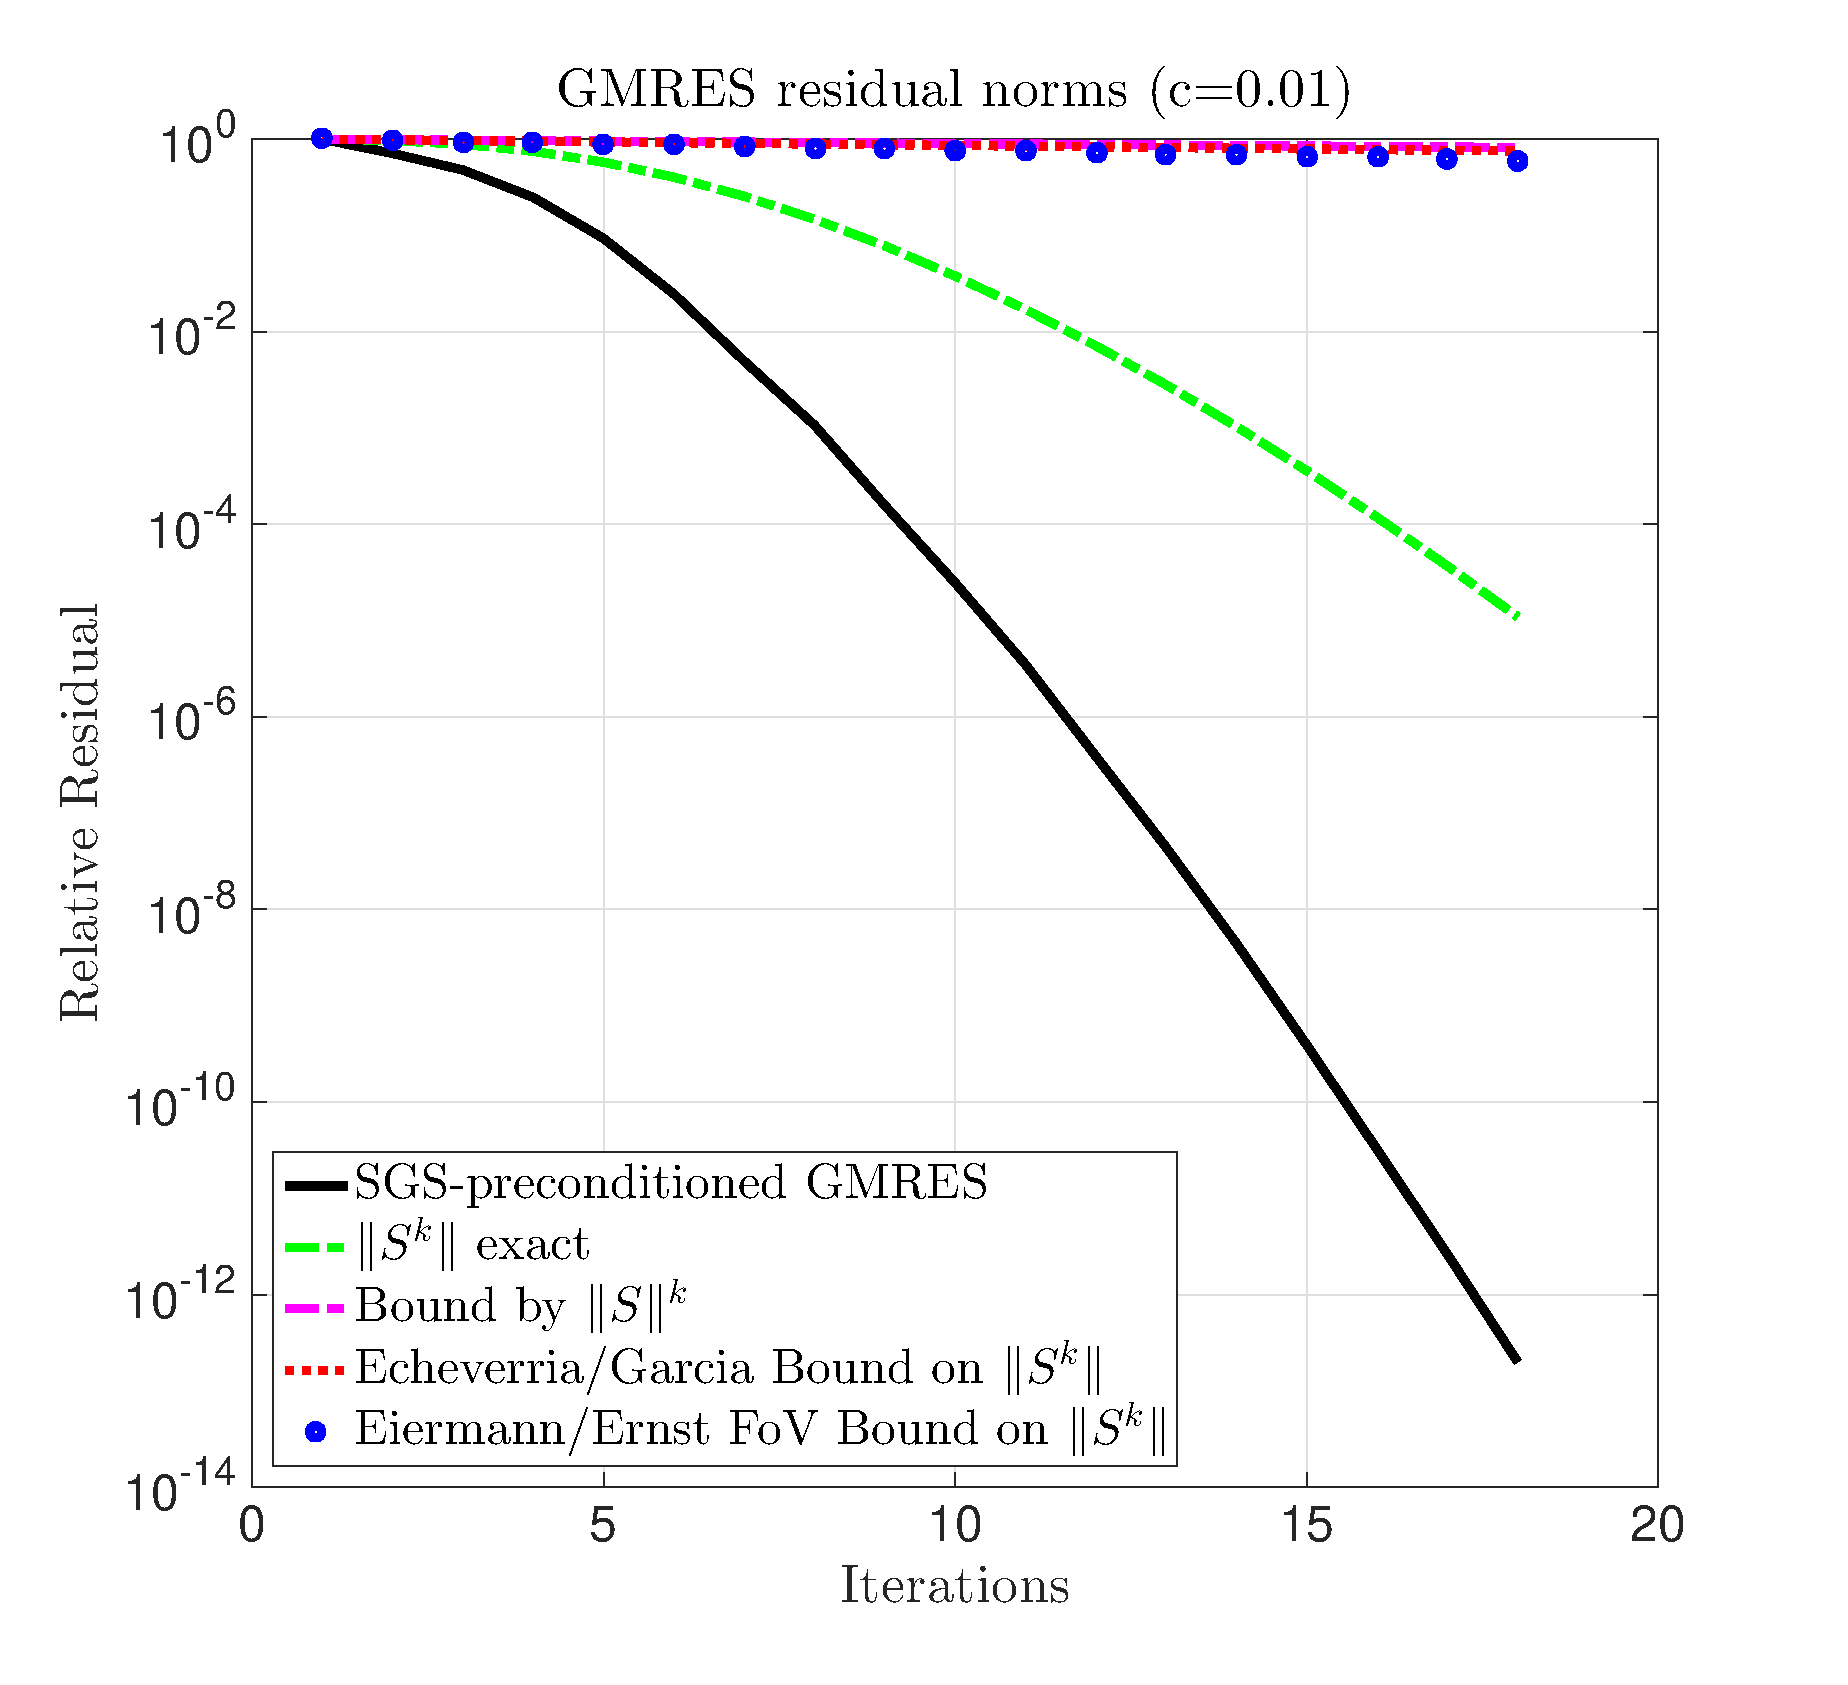
\includegraphics[scale=0.20]{figures/Bounds_1e_neg2_500}
%\hspace*{-2em}
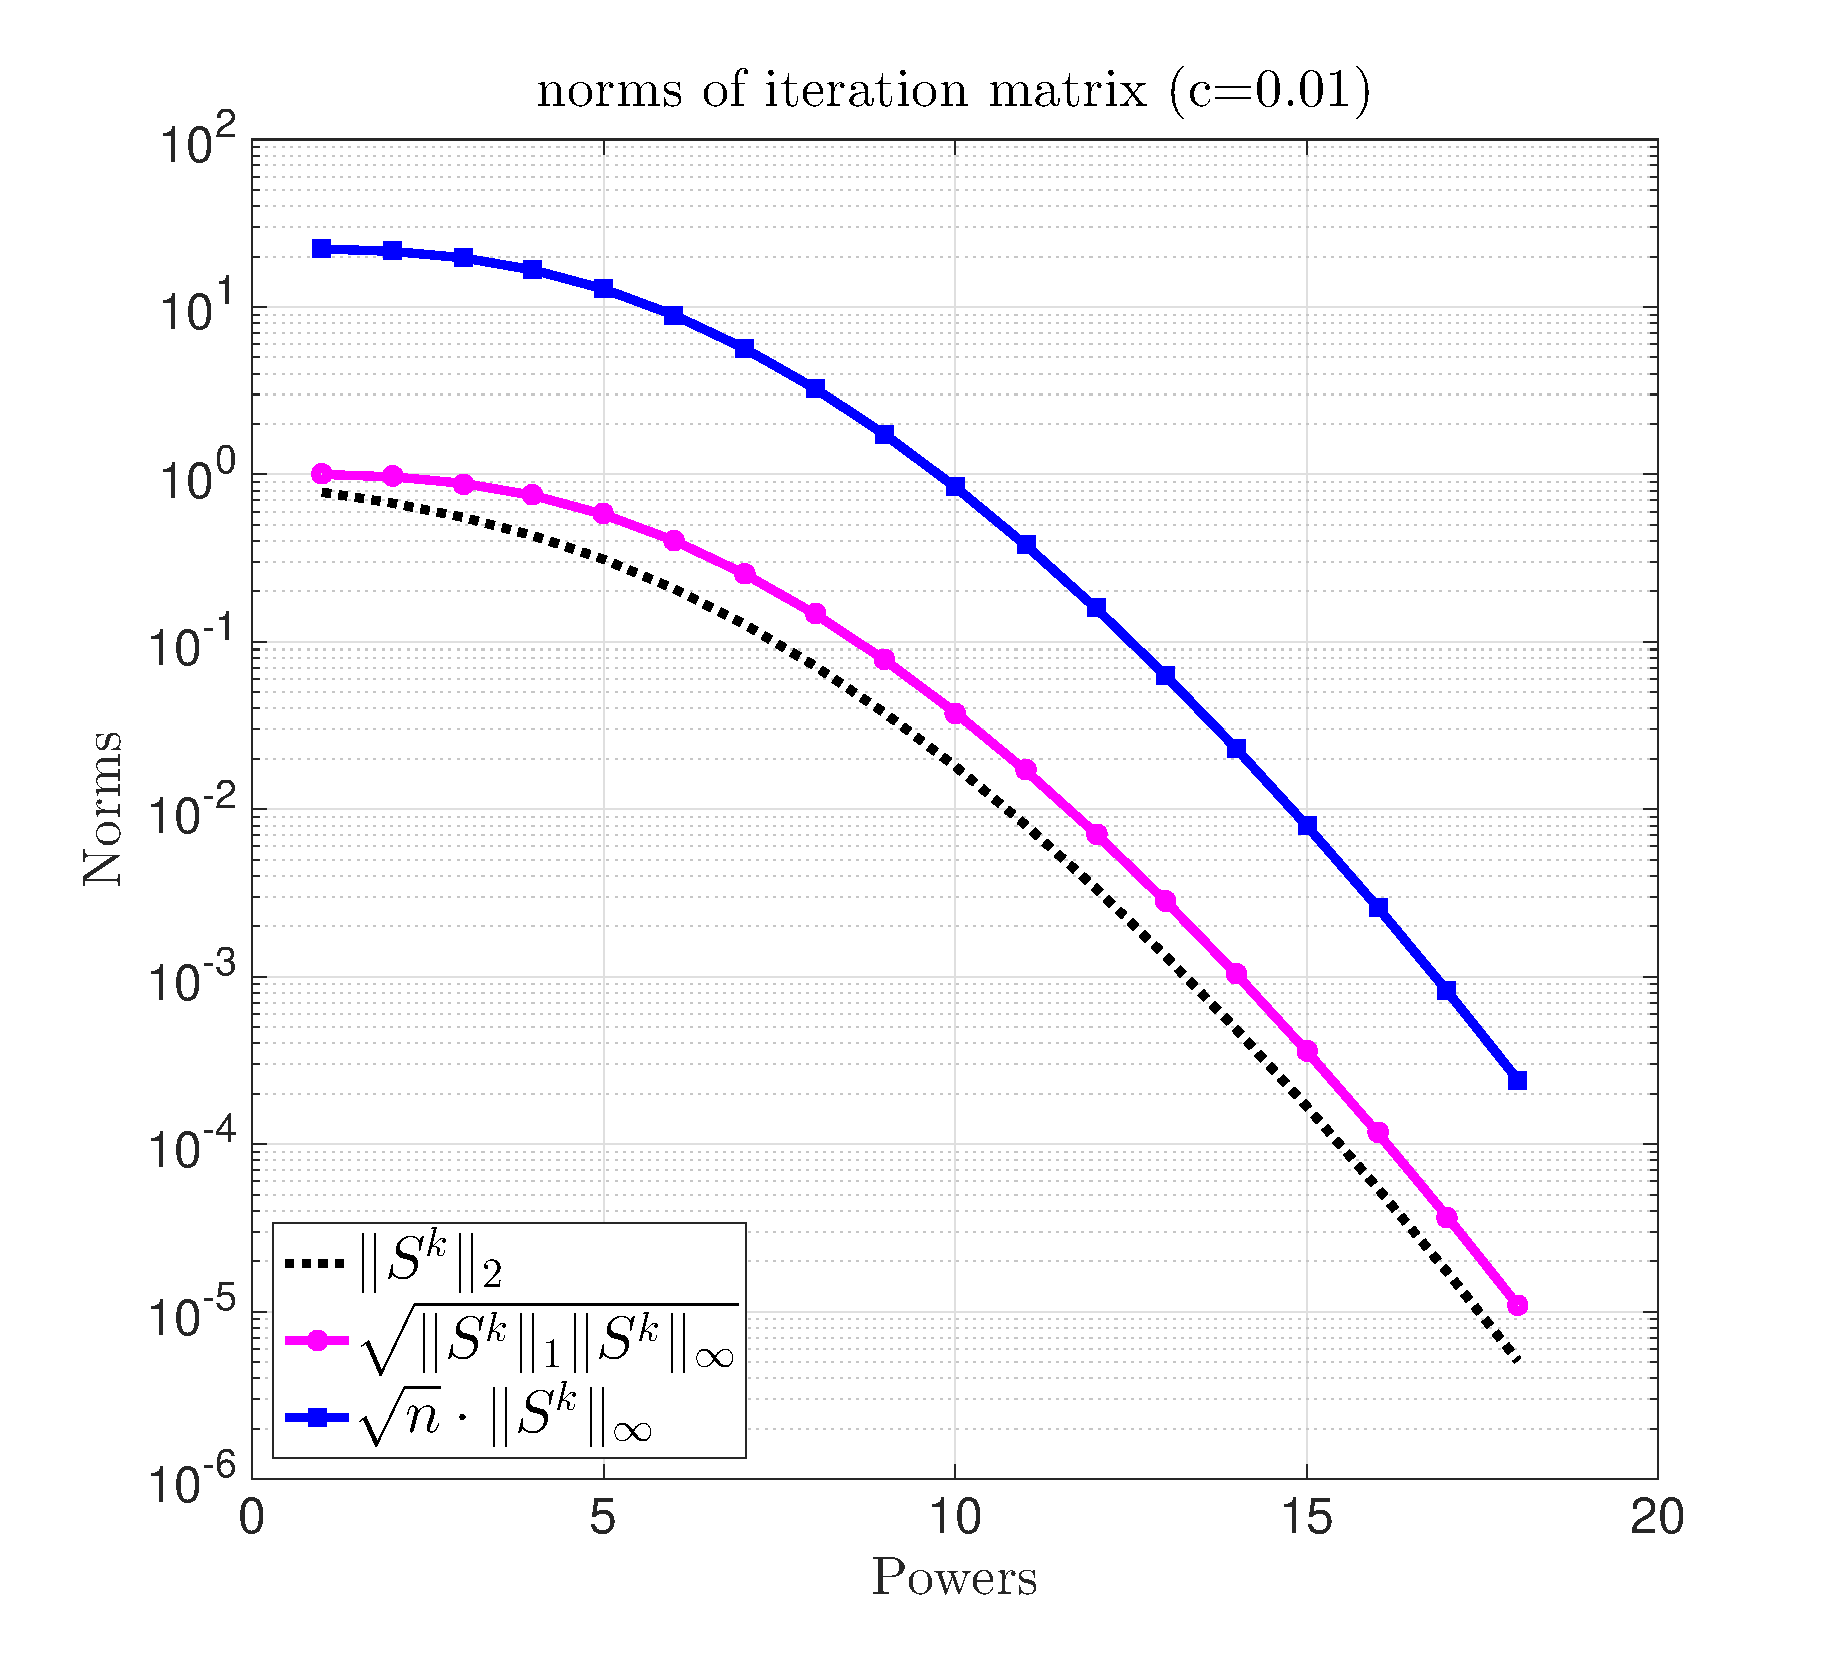
\includegraphics[scale=0.20]{figures/norm_1e_neg2_500_prec}\\
%\vspace*{-1em}
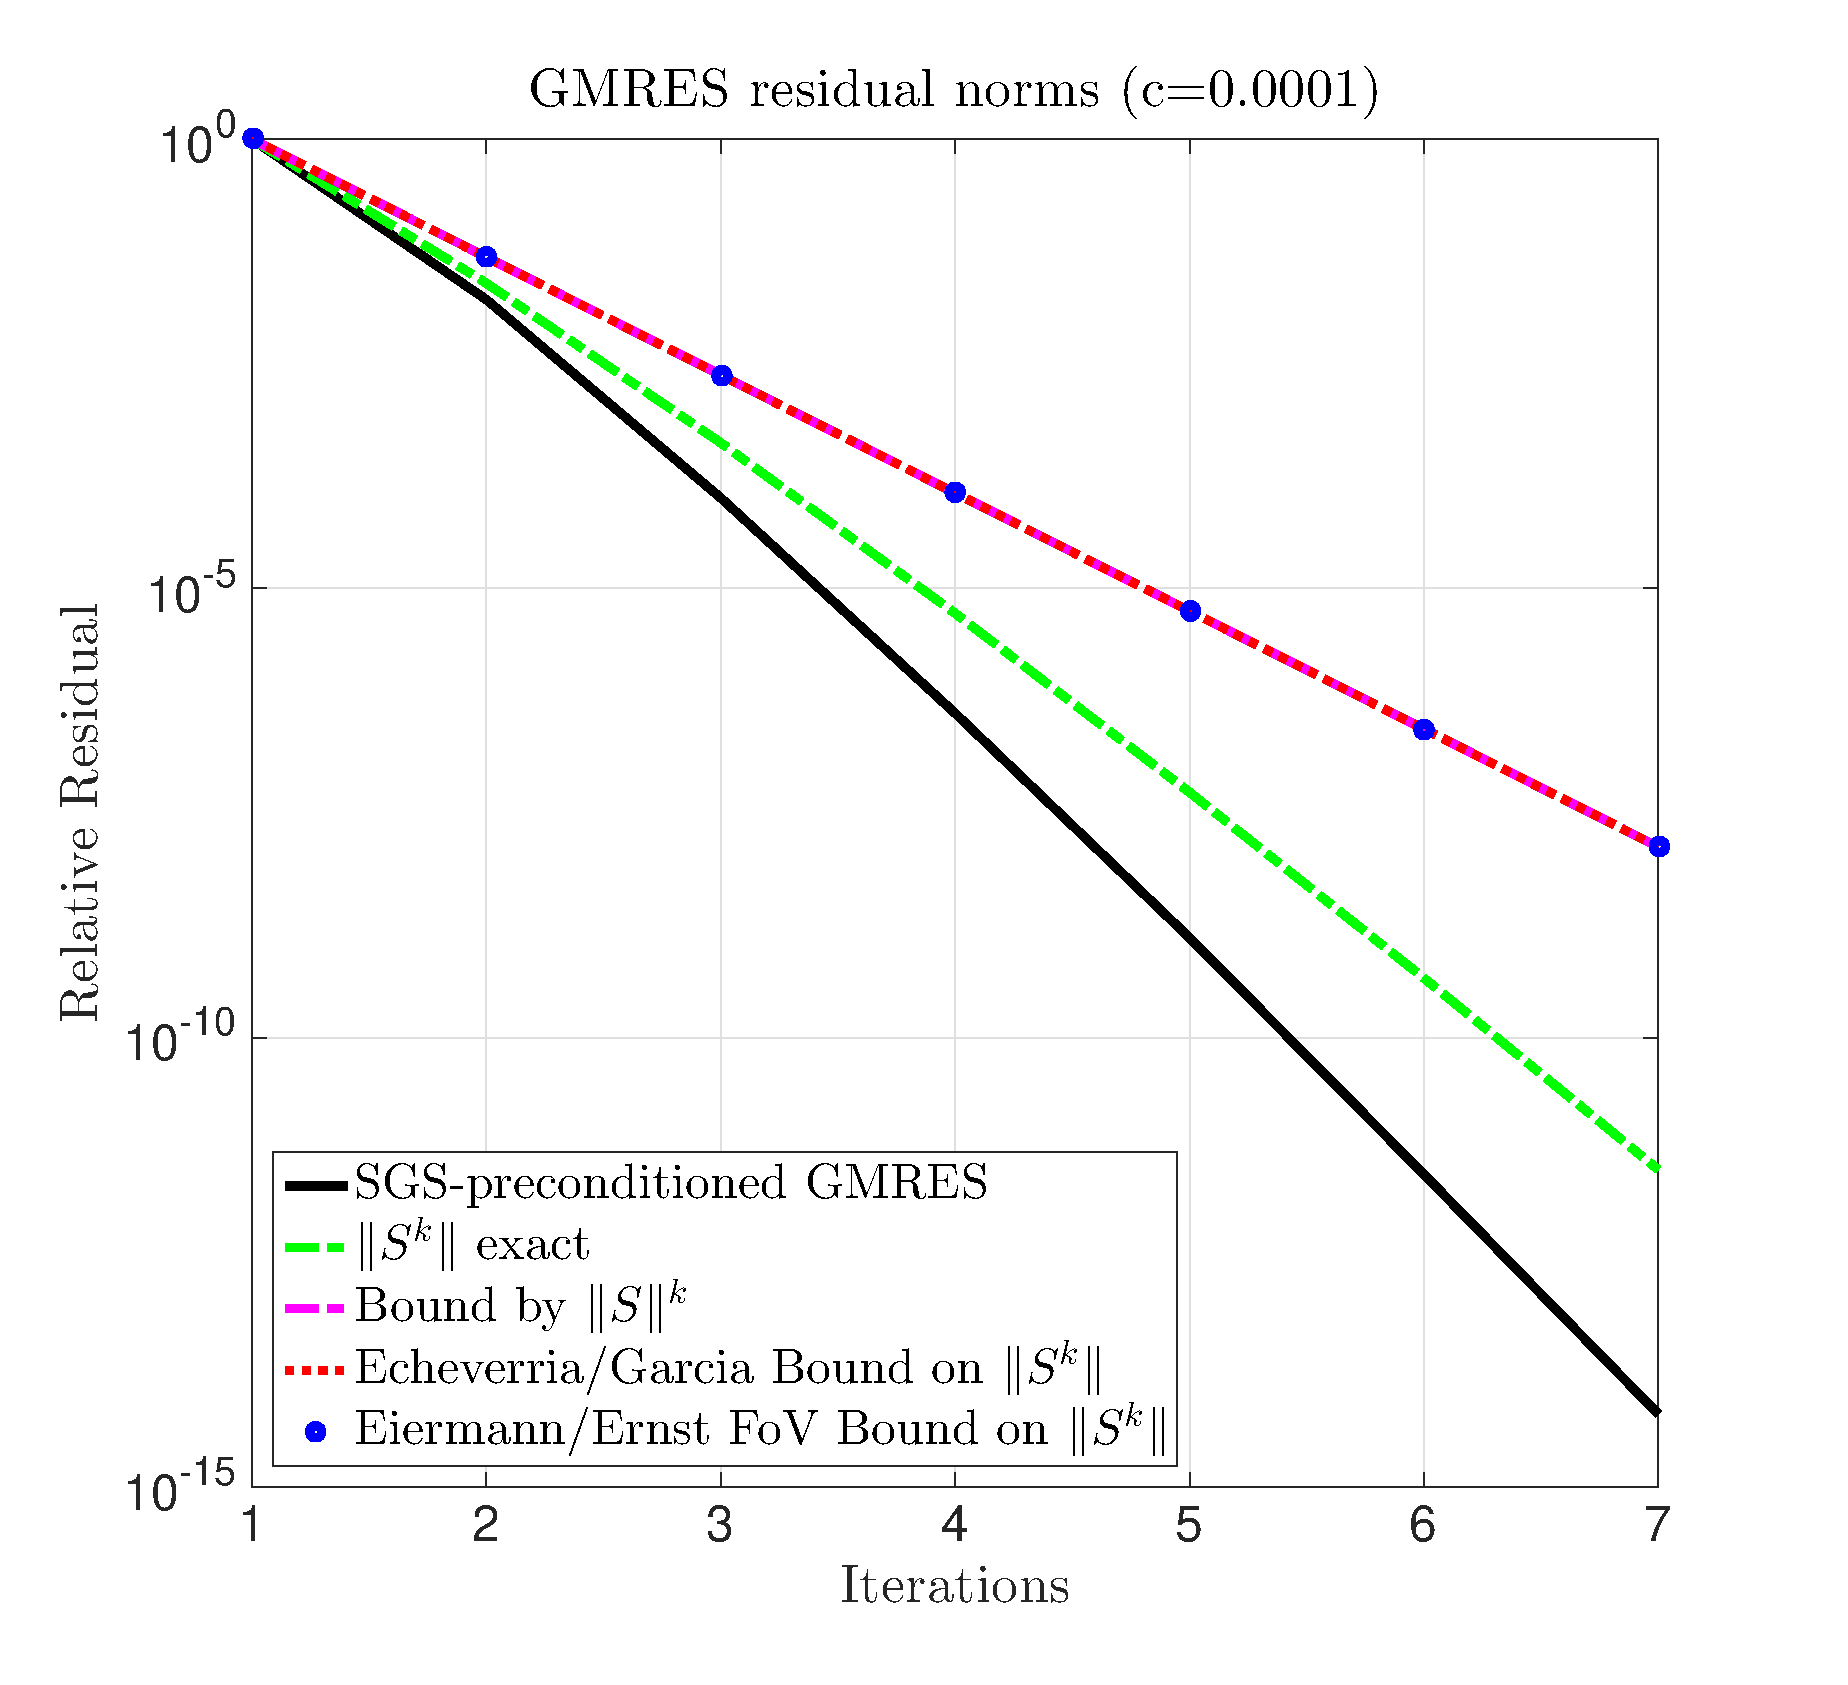
\includegraphics[scale=0.20]{figures/Bounds_1e_neg4_500}
%\hspace*{-2em}
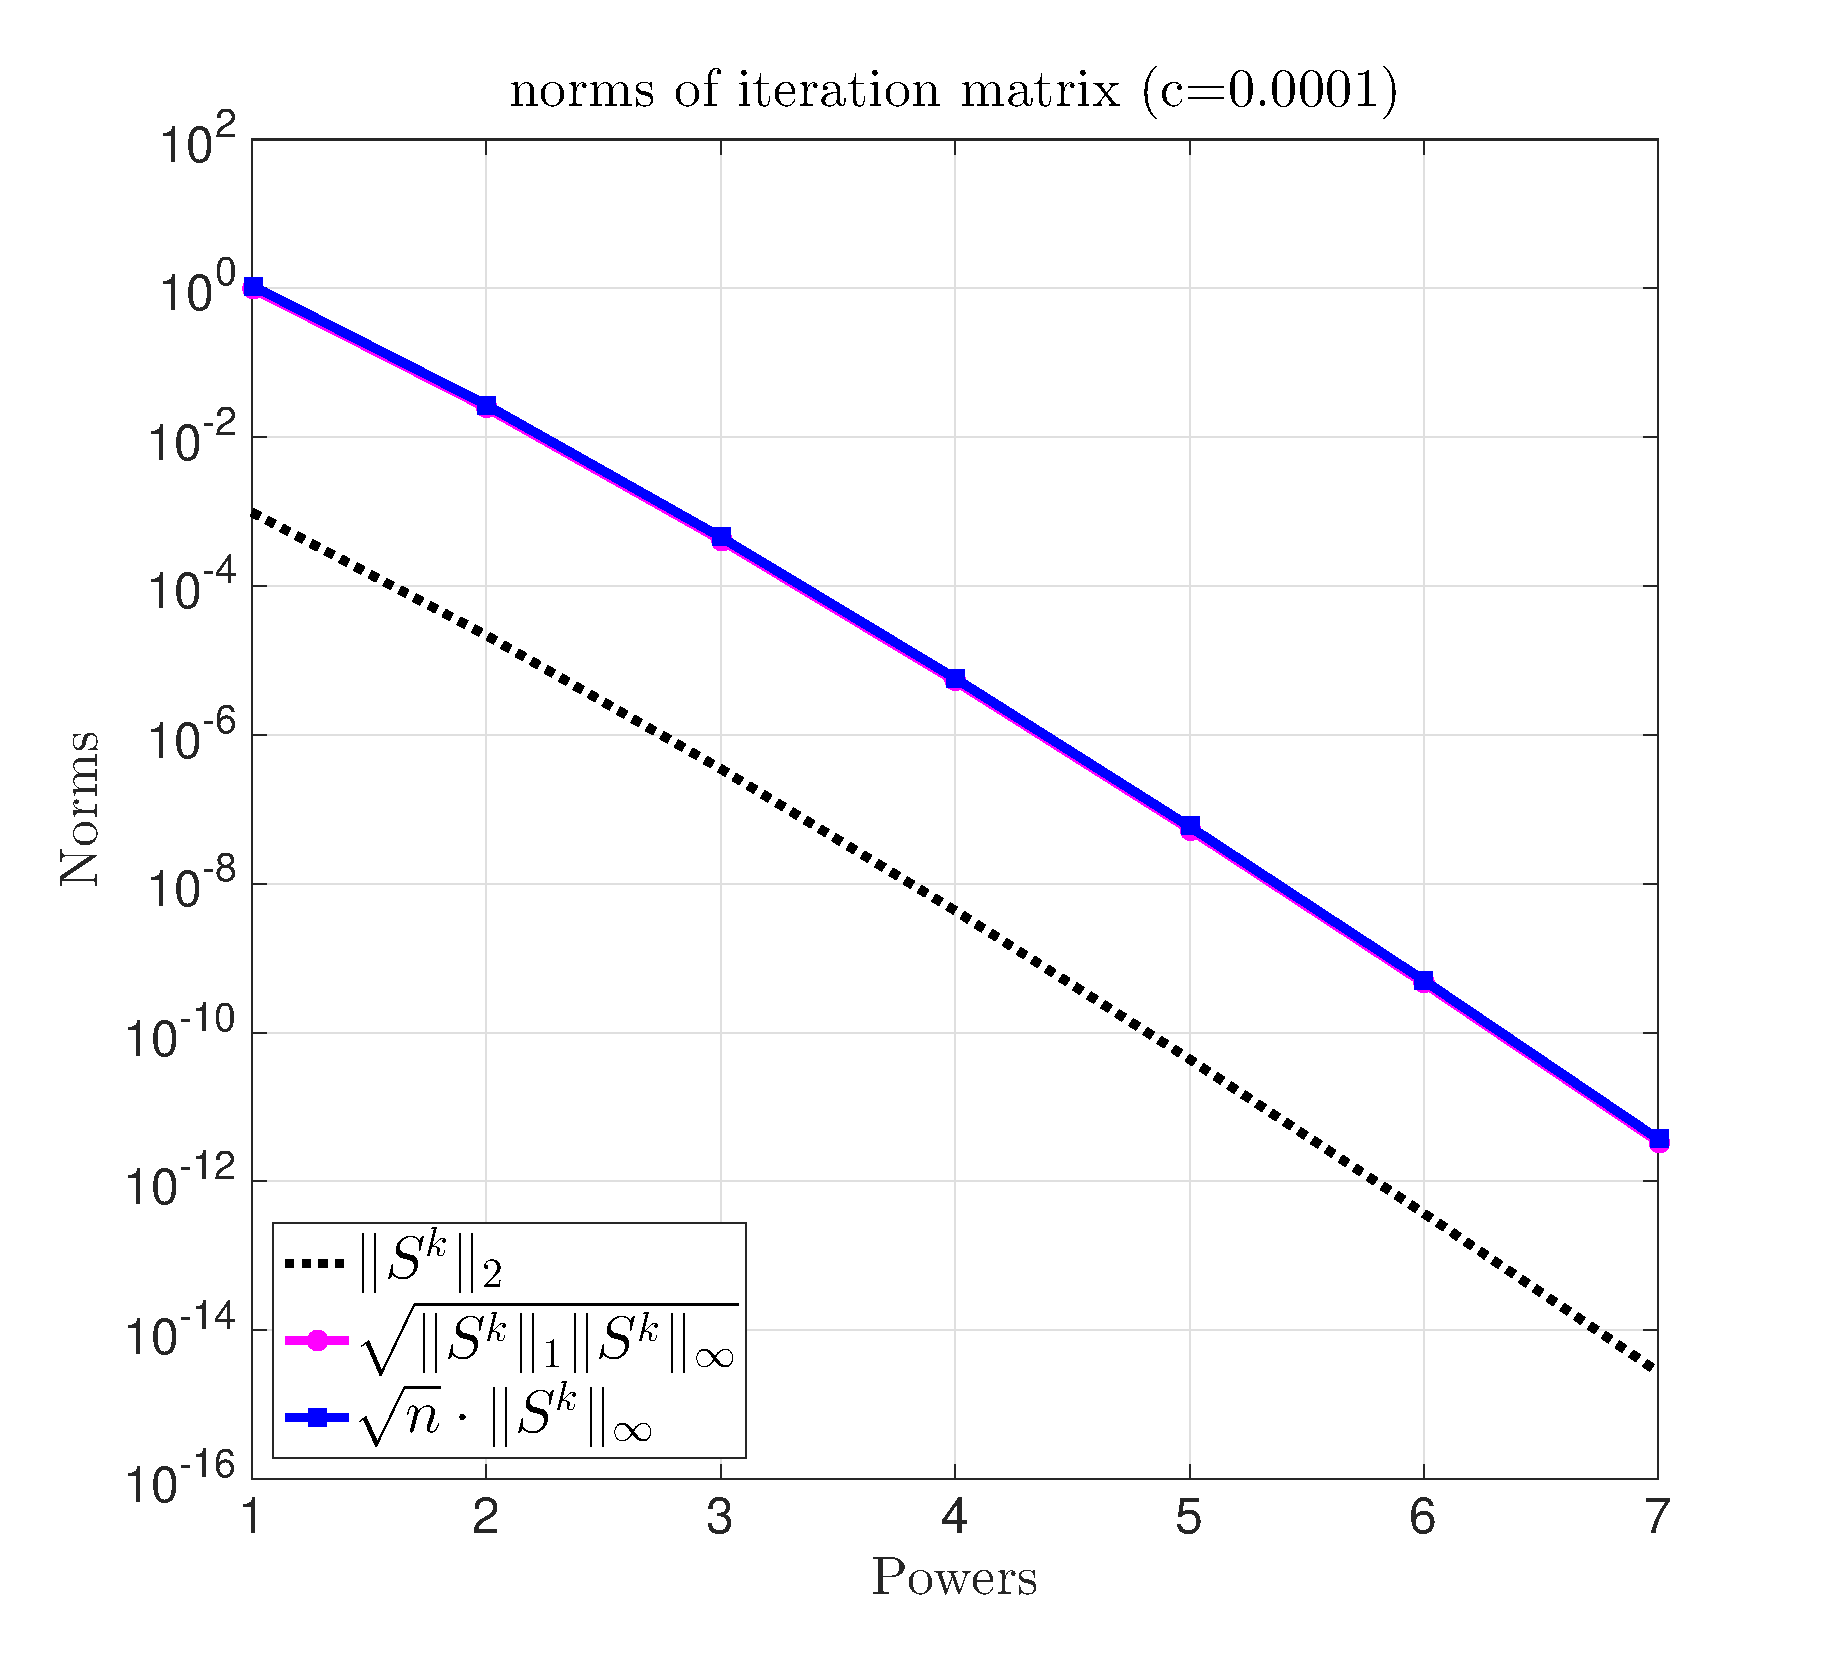
\includegraphics[scale=0.20]{figures/norm_1e_neg4_500_prec.eps}\\
%\hspace*{-2em}
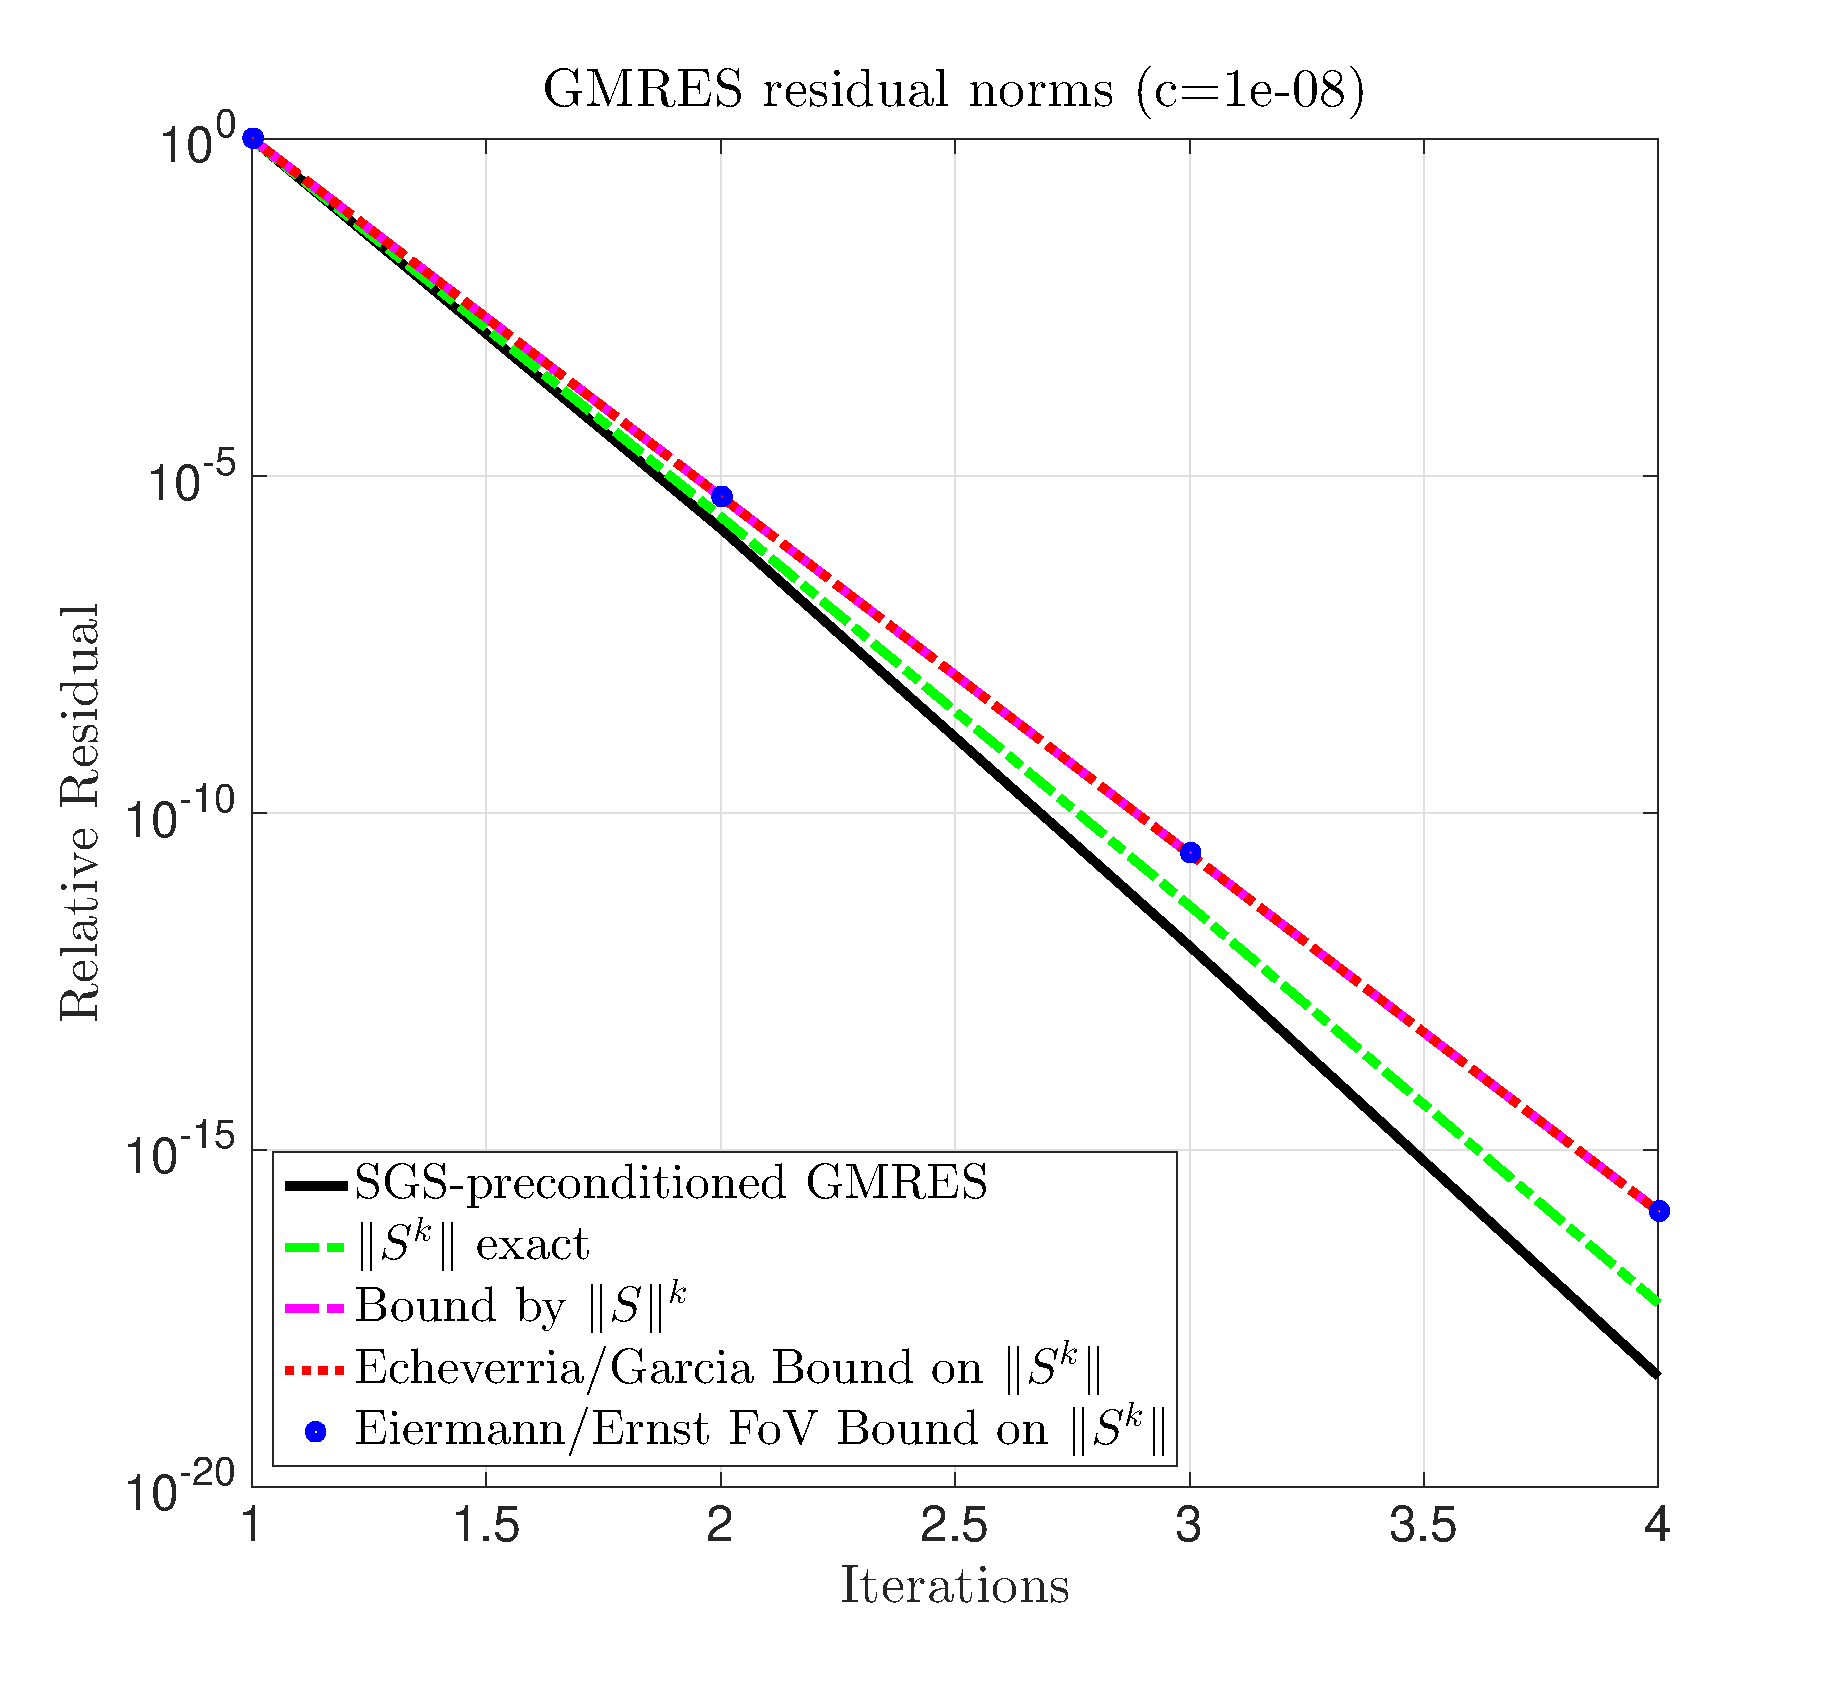
\includegraphics[scale=0.20]{figures/Bounds_1e_neg8_500}
%\hspace*{-2em}
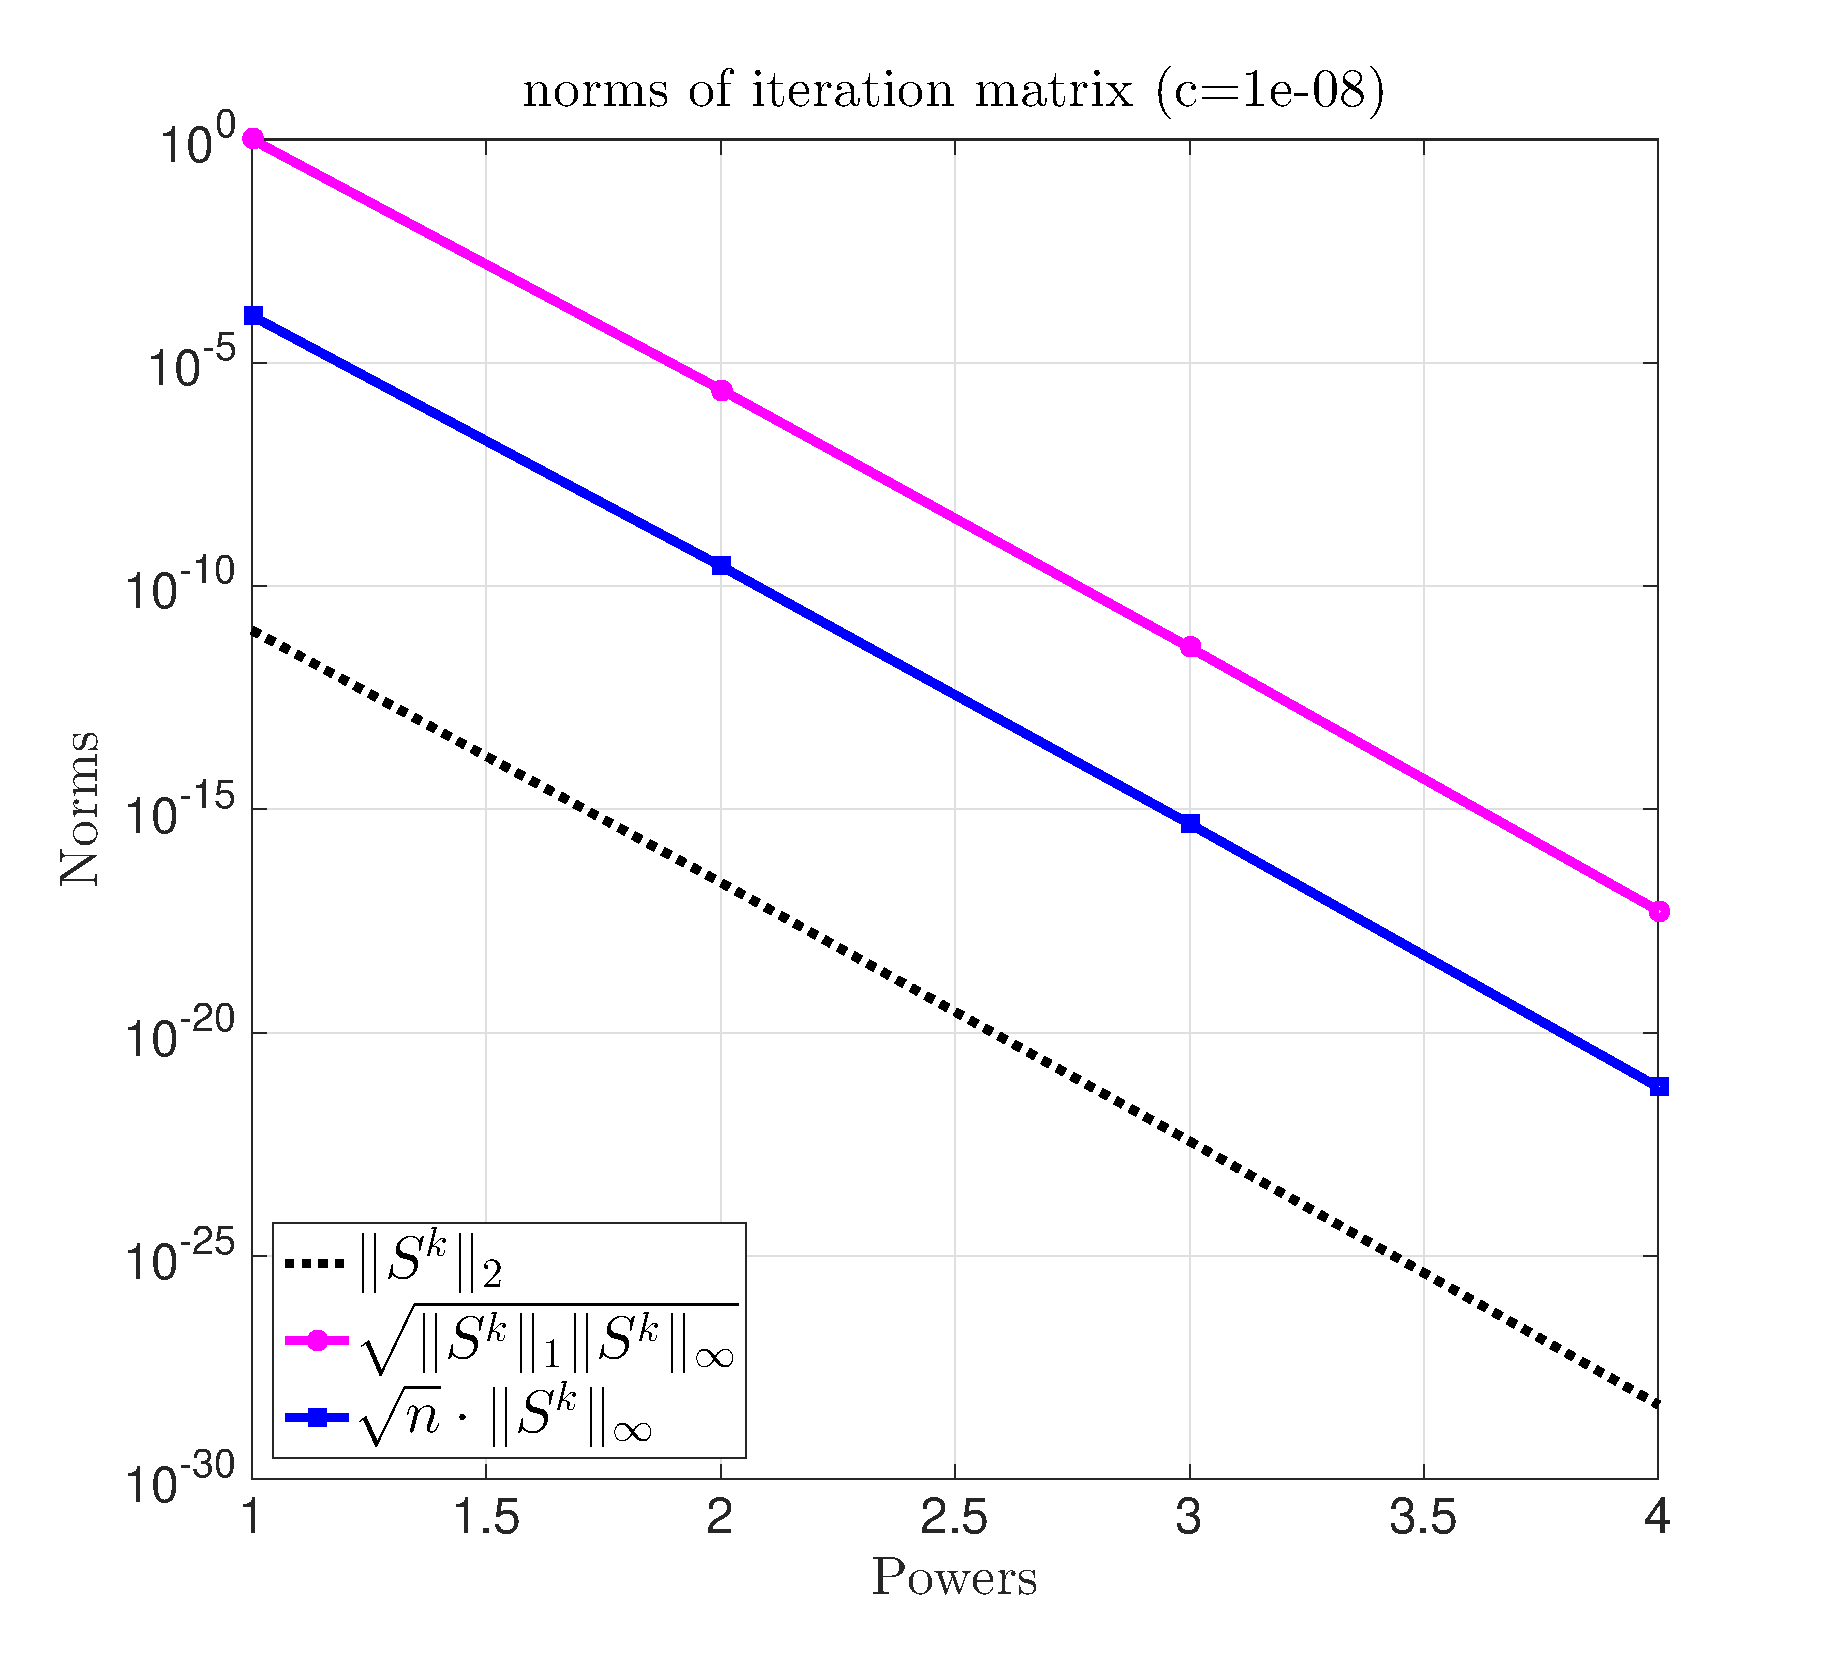
\includegraphics[scale=0.20]{figures/norm_1e_neg8_500_prec.eps}\\
\caption{Bounds for the GMRES residuals for the SGS-preconditioned system of
size $500$ for different values of $c$. Two upper bounds on the $2$-norm are
shown on the right side.}
\label{fig:1D:flow_follow}
\end{figure}

Figure~\ref{fig:1D:flow_follow} also shows that this approach also works for
the SGS method. The figure also shows that we can achieve a bound on the 2-norm
if we manage to bound the $\infty$-norm and the $1$-norm since for every matrix
$\X$ with nonegative entries we have~\cite{GolVan13}
\[
\|\X\|_2\leq\sqrt{\|\X\|_1\|\X\|_{\infty}}.
\]
